% !Mode:: "TeX:UTF-8"

%%UTF-8
\documentclass[twoside]{nputhesis}
%\documentclass[oneside]{nputhesis}

\usepackage{amsmath}
\usepackage{amsfonts}
\usepackage{booktabs}
\usepackage{multirow}
\usepackage{graphicx}
\usepackage{subfig}
\usepackage{stmaryrd}
\usepackage{standalone}
\usepackage{tabularx} % for 'tabularx' environment
\usepackage[numbers,sort&compress]{natbib}
\usepackage[section]{placeins}

\usepackage{lipsum}

\usepackage{color}

\usepackage{tikz}
\usetikzlibrary{matrix,chains,positioning,decorations.pathreplacing,arrows}

\usepackage{algorithm}
\usepackage{algorithmicx}
\usepackage{algpseudocode}
\usepackage{amsmath}
\usepackage{amssymb}
\usepackage{mathrsfs}
\usepackage{ulem}
\usepackage{bm}
\floatname{algorithm}{算法}
\renewcommand{\algorithmicrequire}{\textbf{输入:}}
\renewcommand{\algorithmicensure}{\textbf{输出:}}
% 增加 \ucite 命令使显示的引用为上标形式
% \newcommand{\ucite}[1]{$^{\mbox{\scriptsize \cite{#1}}}$}
% \newcommand{\upcite}[1]{\textsuperscript{\textsuperscript{\cite{#1}}}}
\newcommand{\ucite}[1]{{\textsuperscript{\cite{#1}}}}
\newcommand{\sWuhao}{\fontsize{10.5pt}{10.5pt}\selectfont}      % 五号, 单倍
\newcommand\equref[1]{公式(\ref{#1})}

\usepackage{enumitem}
\setitemize[1]{itemsep=0pt,partopsep=0pt,parsep=\parskip,topsep=5pt}

\def\final{0} % 1--明评,0--盲评


\usepackage{multirow}
\schoolno{10699}
\classno{TP27}
%\secretlevel{}
\title[A Research on Radar Signal Classification using Deep Learning Based Techniques]{基于深度学习的\\雷达信号分类算法研究}
\applydate[January 2018]{2018~年~1~月}
\major[Control Theory and Control Engineering]{控制理论与控制工程}

% \support{本文研究得到青年科学基金项目“基于子模优化的远程预警传感器管理研究”(基金编号:61503305)资助。}

\begin{document}
\ifx\final\undefined

\else
    \if\final1
        \author[Zhang Zhishan]{张治山}
        \authorno{2015201518}
        \supervisor[Pan Quan]{潘泉}
    \else
        \author[\hspace{20 mm}]{\hspace{20 mm}}
        \authorno{\hspace{20 mm}}
        \supervisor[\hspace{20 mm}]{\hspace{20 mm}}
    \fi

    \makecover
    \frontmatter
    % 中文摘要
    % 中文摘要
\begin{abstract}
	% 中文 \lipsum[2-3]

	% 摘要——学位论文的简短陈述,应说明该研究工作的目的意义、研究方法、研究成果等,其重点是研究成果,摘要字数一般为硕士论文700~1000字
	\begin{keywords}
		深度学习, 天波超视距雷达, 地海杂波识别, 辐射源分类, 未知分类, 卷积神经网络
	\end{keywords}
\end{abstract}
    % 英文摘要
    % 英文摘要
\begin{Abstract}
	\lipsum[1-4] 
	\begin{Keywords}
		English, Abstract
	\end{Keywords}
\end{Abstract}

    \tableofcontents

    \mainmatter
\fi
% 正文内容
 \chapter{绪论}
\section{引言}
而是
\section{天波超视距雷达地海杂波识别}
短发
\section{辐射源类别识别}

辐射源的快速、准确和鲁棒的自动目标识别在现代军事中的作用十分重要,自动目标识别算法需要可以准确区分出已知目标和未知目标,同时可以正确的对于已知目标进行分类。我们需要在未收集大量数据的前提下,可以迅速的识别出新的目标。与传统的利用已知类别的样本进行训练测试的机器学习算法不同,我们这个问题是在Open Set的情况下,将需要考虑将输入识别为未知的情况。本文利用深度卷积神经网络与支持向量机进行结合,以雷达信号的模糊函数作为训练样本,构建了一个可以对未知分类进行识别的分类器。我们利用实际数据进行验证,证明我们的分类器具有很强的准确性。
随着科学技术的进步,现代战场形势瞬息万变,信息对抗在现代军事中的作用越来越重要。纵观整个 20 世纪所爆发的两次世界大战和数次局部战争、21 世纪初的美阿、美伊之战以及最近闹得沸沸扬扬的韩国的萨德事件,无一不昭示着现代战争已成为电子战的“天下”,电子战技术也在历次实战演练中逐渐成熟。电子战也称电子对抗,包括电子侦察、电子攻击和电子防护三个方面。电子侦察主要指从敌方雷达及其武器系统获取有用信息,通过雷达辐射源个体识别,可以对战场环境中敌我双方雷达辐射源的分布情况实施侦察,提供更加全面的、精确的电磁斗争与武器的态势,进行有效的战场指挥与决策,雷达辐射源个体识别已成为当前电子战特别是电子侦察领域的研究热点和难点。然而由于辐射源的特征未知、信号波形日趋复杂、战时电磁环境恶劣,给辐射源的精确识别带来了越来越严峻的挑战。

在雷达辐射源信号特征挖掘方面,己有很多学者作了大量研究工作,在上世纪70年代国外相关研究人员就开始了该部分的研究,该部分研究可以分为两个阶段:
第一阶段为辐射源基本参数特征研究。对于原始信号特征直接求取其载波频率、脉冲宽度、脉冲幅度、到达角度和到达时间等信息,利用其中一个或多个作为特征向量。这种情况主要是应用于电磁环境相对单一、辐射源类别较少、信号形式单一、雷达参数固定的早期。

第二阶段自20世纪90年代以来,西方的军事强国开始研究雷达辐射信号的脉内特征,相继提出了了多种分析雷达信号脉内特征的方法。有代表性的工作有:时域波形分析法、谱相关法、基于专家知识信号处理法、时频综合法、小波分析法、信息理论准则与聚类技术综合法、脉内瞬时频率特征与累积法、信号的分型特征等。

国内对雷达辐射源个体识别技术的研究始于上世纪 80 年代初,虽然起步较晚,但受到了军方的高度重视,在“九五”、“十五”和“十一五”国防预研中给予了大力资助。在脉内特征挖掘方面,毕大平提出易于工程实现的脉内瞬时频率提取技术;张葛祥提出了雷达辐射源信号的小波包特征、相像系数特征、熵特征、粗集理论、信息维数和分形盒维数;朱明提出了基于原子分解的特征、基于Chirplet原子的特征、时频原子特征;普运伟提出了瞬时频率派生特征、模糊函数主脊切面特征;陈稻伟提出了符号化脉内特征、围线积分双谱特征等;余志斌提出的局域波分解、小波脊频级联特征。

另一方面,雷达辐射源识别是一个典型的分类问题,其主要思路为在得到辐射源信号的特征表示之后,借助有效的分类算法来实现特征空间到决策空间的转换,从而确定信号的所属类别。大量的分类算法被成功运用于雷达辐射源识别中,如模板匹配、神经网络、支持向量机等。一般被应用于该领域的有三种分类方法,一种是判别型分类器,其需要在学习过程中最优化某种目标函数;另一种为生成模型分类器,其主要是基于先验概率和类别条件概率密度进行估计,如线性判别分类器、K最近邻等;第三种是决策树分类算法,通过人类专家的先验知识进行分类,如ID3、C4.5算法。

\section{论文研究内容及结构}
% !Mode:: "TeX:UTF-8"

\chapter{深度卷积神经网络}
\label{sec:network}
\section{引言}

人工神经网络\ucite{hebb2005organization}是一种通过模仿大脑神经元行为进行信息处理的数学模型,但其无法承受大规模的参数和训练样本并且具有泛化能力差等问题。Fukushima\ucite{fukushima1982neocognitron}于1982年首次提出了卷积神经网络模型,Lecun 等人对神经网络传统算法在训练上面临的计算复杂度高等问题进行了改进,提出了基于梯度下降的优化算法\ucite{lecun1998gradient} 和BP算法\ucite{lecun1989backpropagation}。2003年,Simard对卷积神经网络进行了简化\ucite{simard2003best}。Hinton 在2006年的两篇文章\ucite{hinton2006reducing,hinton2006fast}可以作为深度学习(Deep Learning, DL)正式提出的里程碑。Ciren等人\ucite{ciresan2011flexible}在2011年对神经网络进行改造使其可以通过GPU训练计算,并在大量的图像数据集对深度学习算法进行了测试,且都取得了最好的成绩。其在工业界以及学术界掀起了巨大的浪潮,被应用于语音识别\ucite{hinton2012deep}、图像识别\ucite{krizhevsky2012imagenet}和自然语音处理\ucite{collobert2011natural}等各种方面。专门用于深度学习的芯片不断问世,例如谷歌公司的TPU\ucite{jouppi2017datacenter},大大提高了深度学习的应用场景。

深度神经网络模型是一种非常强大的深度学习模型,它同时可以处理有监督和无监督学习任务。并且随着科技的发展,数据量越来越大,计算机并行能力也有了很大的提高。针对海量数据,简单的线性模型由于无法充分利用计算能力,不再适用,可以预见在将来会有越来越多的工作应用到深度学习。目前,其内涵已经超出了传统的多层神经网络,甚至机器学习的范畴,逐渐朝着人工智能的方向快速发展\ucite{silver2017mastering}。

本章安排如下:\ref{sec:network_classification}节对深度学习的基本分类进行了介绍,\ref{sec:neural}节详细地阐述了传统人工神经网络结构的定义和神经元之间信息传递的过程,\ref{sec:cnn}节对本文主要运用的深度卷积神经网络的特性进行了介绍,\ref{sec:network_summary}节进行本章总结。

\section{基本分类}
\label{sec:network_classification}
传统上可以把深度学习分为卷积神经网络、递归神经网络(Recurrent Neural Networks, RNN)、长短时记忆网络(Long short-term memory, LSTM)、深度信念网络(Deep Belief NetWorks, DBN)、自编码器、稀疏编码(Sparse Coding)、受限玻尔兹曼机(Restricted Boltzmann Machine, RBM)等。

其中卷积神经网络是最流行的一种深度学习模型,通过使用卷积层极大地减少了中间层的参数数目,使学习效率更高并减少过拟合,同时卷积操作独有的局部感受野(local receptive fields)、共享权重(shared weights)和池化(pooling)三种特性也是处理序列元素分类识别的很重要的一点,权重共享策略减少了需要训练的参数,相同的权重可以让卷积核不受信号位置的影响来检测信号的特性,使得训练出来的模型泛化能力更强;池化运算可以降低网络的空间分辨率,从而消除信号的微小偏移和扭曲。

递归神经网络是一种包含循环的,允许信息持久化的神经网络模型。传统的前馈神经网络中,单独的输入完全确定了余下层的神经元的激活值。而递归神经网络对的隐层和输出层的神经元的激活值不仅由当前的网络输入决定,而且包含了前面的输入的影响。长短时记忆网络是一种特殊的递归神经网络,主要用于解决递归神经网络前期模型难以训练的问题。其通过刻意设计的单元结构,在递归神经网络的基础上添加了元胞状态(cell state)用来保存长期的状态,然后通过门函数来控制此长期状态。

深度信念网络是一个概率生成模型,是由多个受限玻尔兹曼机组成,这些网络被“限制”为一个可见层和一个隐层,层间存在连接,但是层内的单元间不存在连接,通过训练隐层单元来捕捉在可见层表现出来的高阶数据的相关性。

通过对以上几种最常用的深度学习方法的介绍,易知卷积神经网络最适合处理本文这种静态类型的数据,循环或者说是不同时刻的输入对地海杂波类型的识别并没有提高,故递归神经网络和长短时记忆网络显然不适合本问题。另一方面,深度信念网络的生成模型并不关心不同类别之间的最优分类面的位置,故其用于分类问题时,分类精度没有判别模型高。且其学习的是数据的联合分布,相比其他算法具有更高的复杂性。

\section{传统人工神经网络结构}
\label{sec:neural}
人工神经网络是一种模拟大脑神经系统的算法,其可以从海量的训练样本中学习到一个权重函数,用来进行模式识别、分类等。神经网络主要是将许多个单一神经元(也称作感知器)连接在一起,一个神经元的输出就可以是另一个神经元的输入,形成一个有向无环的网络结构。
首先介绍单一神经元的结构,如图\ref{fig:neural}所示,神经元一般具有多个输入$x=[x_1,x_2,\dots,x_n] $,这些输入可以取0和1中的任意值。神经元对每一个输入有权重$w=[w_1,w_2,\dots,w_n] $ 和一个总的偏置$b_0$ ,其输出为:
\begin{equation}
y = f(w\cdot x + b_0),
\label{equ:neural}
\end{equation}
其中, $f$为该神经元的激活函数。

\begin{figure}[hbt]
  \centering   \sWuhao
  \includestandalone{figures/networks/neural}
  \caption{神经元}
  \label{fig:neural}
\end{figure}

上述多个神经元分层互联即可形成神经网络,图\ref{fig:network}是一个简单的神经网络,其中圆圈表示神经网络的节点,也即神经元。
对于一个具有$n_l$层的神经网络,如将第$ l $层用 $ L_l$表示,则有最左边的一层$  L_1$为输入层,最右的一层$ L_{n_l} $为输出层。由于不能在训练样本集中观测到中间所有节点的值,故将这些层称做隐层。
本例中网络的层数$n_l=3$,输入层具有4个输入单元,隐层具有5个隐层单元,输出层只有一个输出单元。

\begin{figure}[hbt]
\centering
\sWuhao
\includestandalone{figures/networks/network1}
\caption{神经网络}
\label{fig:network}
\end{figure}

根据输入 $x_i$求解输出$y$的主要过程为前向传播。
用$ w^{(l)}_{ij}$表示第 $ l $层的第 $ j$ 单元与第 $l+1 $层的第$i$ 单元之间的权重,$ b^{(l)}_i $是第$l$层中第$i$ 单元的偏置项。
因此,$w^{(l)}$为第$l$层权重组成的向量,$ w^{(1)} \in \mathbb{R}^{4\times 3}$ , $ w^{(2)} \in \mathbb{R}^{1\times 5}$ 。
根据图\ref{fig:neural}和\equref{equ:neural}可以知道每个神经元节点的输出是经过激活函数的激活值,可以用$ y^{(l)}_i$ 表示第$  l $层的第 $ i$ 单元的输出值。
当$  l=1$ 时,$  y^{(1)}_i$为就是第$  i $个输入值,也即有$  y^{(1)}_i = x_i $。
当权重已知时,可以根据\equref{equ:neural}求解此传播过程,进而求解最终的输出值$y$。
从$L_1$层到$L_2$层的过程为:
\begin{align}
  y_1^{(2)} &= f(w_{11}^{(1)}x_1 + w_{12}^{(1)} x_2 + w_{13}^{(1)} x_3 + w_{14}^{(1)} x_4 + b_1^{(1)}),  \\
  y_2^{(2)} &= f(w_{21}^{(1)}x_1 + w_{22}^{(1)} x_2 + w_{23}^{(1)} x_3 + w_{24}^{(1)} x_4 + b_2^{(1)}),  \\
  y_3^{(2)} &= f(w_{31}^{(1)}x_1 + w_{32}^{(1)} x_2 + w_{33}^{(1)} x_3 + w_{34}^{(1)} x_4 + b_3^{(1)}),
\end{align}
\begin{align}
  y_4^{(2)} &= f(w_{41}^{(1)}x_1 + w_{42}^{(1)} x_2 + w_{43}^{(1)} x_3 + w_{44}^{(1)} x_4 + b_4^{(1)}),  \\
  y_5^{(2)} &= f(w_{51}^{(1)}x_1 + w_{52}^{(1)} x_2 + w_{53}^{(1)} x_3 + w_{54}^{(1)} x_4 + b_5^{(1)}).
  \label{equ:fp1}
\end{align}
根据同样的计算过程可以得到:
\begin{equation}
  y = y_1^{(3)} =  f(w_{11}^{(2)} y_1^{(2)} + w_{12}^{(2)} y_2^{(2)} + w_{13}^{(2)} y_3^{(2)} + w_{14}^{(2)} y_4^{(2)} + w_{15}^{(2)} y_5^{(2)} + b_1^{(2)}).
  \label{equ:fp2}
\end{equation}
把\equref{equ:fp1}代入\equref{equ:fp2}就可以计算得到输入$x_i$与输出$y$之间的关系。
为了使表达更清晰,用$ z^{(l)}_i $表示第$ l $层第$  i$单元输入加权和,则有:
\begin{equation}
  z_i^{(l)} = \sum_{j=1}^n w^{(l-1)}_{ij} x_j + b^{(l)}_i.
\end{equation}
因此\equref{equ:fp1}变为:
\begin{equation}
  y^{(l)}_i = f(z^{(l)}_i).
\end{equation}
则整个前向传播过程可以简化为:
\begin{align}
  z^{(l+1)} &= w^{(l)} y^{(l)} + b^{(l)}   \\
  h^{(l+1)} &= f(z^{(l+1)}),
\end{align}
其中,$b^{(l)}$为第$l+1$层偏置项组成的向量,$h^{(l)}$为第$l$层各个单元输出值组成的向量。

根据上述计算过程,对于一个具有 $n_l$ 层的前馈神经网络(在网络中没有闭环或者回路),其第$   1 $层是输入层,第$n_l$ 层是输出层,中间的所有隐层 $L_l$ 均与下一层 $L_{l+1}$全连接。
只需逐个计算每一个层中的节点的输出值,然后据此得到下一层的输出值。
一个复杂的神经网络一般会具有多个隐层并且输出层中可以有多个输出单元,
图\ref{fig:network2}的神经网络有三层隐层:$  L_2 $、$ L_3$及 $ L_4$ ,输出层$  L_5 $有三个输出单元。

\begin{figure}[hbt]
  \centering
  \sWuhao
  \includestandalone{figures/networks/network2}
  \caption{具有多个输出单元的神经网络示意图}
  \label{fig:network2}
\end{figure}

\section{深度卷积神经网络}
\label{sec:cnn}
卷积神经网络是深度学习中的一种重要算法,在分类等很多领域具有很大的优势,该方法经常被用于图像识别、语音识别等问题。
卷积神经网络是一种特殊的人工神经网络,由多对卷积层(Convolutional layer)和池化层(Pooling layer),以及全连接层(Full-connected layer)组成。图\ref{fig:cnn_network}为一个典型的卷积神经网络,最左边的为输入层,其中的神经元为输入神经元。最右边的输出层包含有一个或者多个输出神经元,其余的是多组卷积、池化层和有限数量的完全连接的隐层。

网络的前向传播主要是卷积和池化操作,其网络参数的更新采用误差反向传播(Error Backpropagation)算法。相比于传统人工网络,卷积神经网络有以下特点:
\begin{itemize}
  \item 输入为原始数据,对原始数据进行卷积运算,然后提取从最后一步生成的卷积数据的特征,丰富了识别中使用的特征。
  \item 多个卷积核可以利用输入数据中的局部结构,将整个输入空间划分成很小的隐层单元。将各个隐层单元的权重构建得到的卷积核作用于整个输入空间,从而得到特征向量。这种机制不仅大大减少了参数数量同时提高了数据的平移不变性。
  \item 具有超过两个的隐层以及可以逐层初始化模型的参数,通过更多的隐层可以更好地对事物的特征进行学习表达。
\end{itemize}

\begin{figure}[hbt]
  \centering
  \includegraphics[width=13.5cm]{figures/networks/alexnetarchitecture}
  \caption{ AlexNet 卷积神经网络模型\ucite{krizhevsky2012imagenet}}
  \label{fig:cnn_network}
\end{figure}

\subsection{卷积}

深度卷积神经网络在特征提取过程中一个主要操作为卷积,在前向计算过程中,输入的一定区域的隐层的特征向量$x$和滤波器(权重)$w$ 点乘后得到新的特征向量,然后滑过一个个滤波器,以产生输出特征向量。
权重实际上是一个四维张量,第一维$ F $是卷积输入层的特征向量的数量,另一维$ F_p $是卷积输出层的特征向量的数量,另外两维是在宽度和高度方向给出的卷积核的大小,也称作感受野。

传统神经网络的每个输入元素会连接到每个隐层神经元。然而,在卷积神经网络中,只是把输入数据进行小的、局部区域的连接,也即第一个隐层中的每个神经元会连接到一个输入神经元的一个区域。这个输入向量的区域被称为隐层神经元的局部感受野,它是输入向量上的一个小窗口,对每个连接学习一个权重而隐层神经元同时学习一个总的偏置。通过在整个输入频谱数据上交叉移动局部感受野,可以构建起第一个隐层。

感受野允许用一个子集来代替整个输入数据。它的目的是在输入数据中搜索相似的模式,而不管模式在哪里,也即平移不变性。输出图像的宽度和高度也由步长(stride)确定,步长为在进行再次应用卷积运算之前在垂直、水平方向上滑动的像素的数目。以图\ref{fig:conv}展示的二维卷积操作来介绍卷积运算的过程。

\begin{figure}[hbt]
	\centering
  \includegraphics[width=13.5cm]{figures/networks/conv}
	\caption{卷积示意图}
	\label{fig:conv}
\end{figure}

图中的 $R_C$ 为卷积感受野的大小,$S_C$为卷积的步长。
根据输入高度$ T $和宽度$ N $,可以计算输出图像的高度和宽度:
\begin{align}
  N_p&=\frac{N+2P-R_C}{S_C}+1 \;,&
  T_p&=\frac{T+2P-R_C}{S_C}+1.
\end{align}
通常对输入数据进行边界扩充(padding)来使得输入特征图的宽度和高度满足$ N = N_p = T = T_p $,这样当前进步长$ S_C = 1 $ 时,可以得到:
\begin{align}
P&=\frac{R_C-1}{2}.
\end{align}
一个给定的层$ L_n $的卷积运算的计算过程为:
\begin{align}
y_{f\,l\,m}^{(\nu)}&=\sum^{F_\nu-1}_{f'=0}\sum^{R_C-1}_{j=0}\sum^{R_C-1}_{k=0}
w^{(o)f}_{f'\,j\,k}h^{(\nu)}_{f'\,S_Cl+j\,S_Cm+k},
\end{align}
其中$ o $表示网络中的第$ o + 1 $个卷积核。
$\nu \in [0,N-1 ]$ 表示网络中的第 $\nu$个隐层,$f\in[0,F_{\nu+1}-1]$为输入卷积层的第$f$个特征图, $l\in[0,N_{\nu+1}-1 ]$为输入卷积层的第$v$个特征图的宽度单位, $m\in[0,T_{\nu+1}-1 ]$为输入卷积层的第$v$个特征图的高度单位。 因此可以得到 $S_Cl+j\in[0,N_\nu-1 ]$, $S_Cl+m\in[0,T_\nu-1 ]$。于是可以通过添加激活函数计算隐层单元的输出。
考虑到边界填充可以得到:
\begin{align}
h_{f\,l+P\,m+P}^{(\nu+1)}&=f\left(y_{f\,l\,m}^{(\nu)}\right).
\end{align}
每个滤波器只关心数据的部分特征,当出现它学习到的特征时,就会呈现激活态。

\subsection{共享权重和偏置}
如前节所述,每个隐层神经元具有一个偏置和连接到它的局部感受野的权重,对该层的每一个神经元使用相同的权重和偏置,那么第$j$个隐层神经元的输出为:
\begin{equation}
  h_j = f(b+\sum_{m=1}^M w_m y_{j+m}),
  \label{equ:shared_weight}
\end{equation}
其中,$f$是神经元的激活函数,$b$是偏置的共享值,$w_m$是一个共享权重的$1\times M$向量,$y_k$表示位置$k$的输入激活值。
这意味着第一个隐层的所有神经元检测完全相同的特征,只是在输入数据的不同位置,因此卷积网络可以很好地适应数据偏移的情况。

\subsection{池化}
在通过卷积获得了特征之后,下一步希望利用这些特征去做分类。理论上讲,人们可以用所有提取得到的特征去训练分类器,例如Softmax分类器(多分类的逻辑回归分类器),但这样做面临着计算量的挑战,除此以外过多的特征向量,也容易导致过拟合。
由于本文的雷达信号具有一种“静态性”属性,在一个数据区域有用的特征极有可能在另一个区域同样适用。因此,为了描述数据量较多的数据,一个很自然的想法就是对不同位置的特征进行聚合统计,例如,可以计算频谱数据上一段频率范围内的某个特征的最大值(或平均值)。
这些经过采样的统计特征相比使用所有提取得到的特征不仅具有低得多的维度,而且不容易过拟合,在一定程度上会改善结果。这种聚合的操作称为池化。
池化操作是卷积神经网络中一种常用的用来对数据进行降维处理的方法。一般有平均池化和最大池化,主要过程为选取输入特征向量的$F$一个池化感受野$R_P$和步长$S_P$选取其最大或者平均元素来代表该区域,得到输出特征向量$F_p=F$,其中宽度 $N_p<N$,高度 $T_p<T$。在池化操作过程中,一般不考虑输入隐层的边界扩充值,因此在\equref{equ:pool}中存在 $+P$ 这一部分。

给定的第$\nu$个平均池化操作的公式为:
\begin{align}
  y_{f,l,m}^{(\nu)}&=\sum^{R_P-1}_{j,k=0} h_{f,S_Pl+j+P,S_Pm+k+P}^{(\nu)}.
  \label{equ:pool}
\end{align}
最大池化的公式为:
\begin{align}
  y_{f,l,m}^{(\nu)}&=\max_{j,k \in \{0, \ldots, R_P-1\}} h_{f,S_Pl+j+P,S_Pm+k+P}^{(\nu)},
  \label{equ:maxpool}
\end{align}
其中,$\nu \in [0,N-1 ]$ 表示网络中的第 $\nu$个隐层,$f\in[0,F_{\nu+1}-1]$, $l\in[0,N_{\nu+1}-1 ]$ 以及 $m\in[0,T_{\nu+1}-1 ]$。因此有 $S_Pl+j\in[0,N_\nu-1 ]$, $S_Pl+m\in[0,T_\nu-1 ]$。
最大池化是最常用的一种池化方式,本文所用的神经网络结构均使用最大池化。
用$j^{(t)(p)}_{_{f,l,m}},\,k^{(t)(p)}_{_{f,l,m}}$来表示第$t$次批采样在 $l,m$处特征向量图的最大值,则\equref{equ:maxpool} 变为:
\begin{align}
h_{f,l+P,m+P}^{(t)(\nu+1)}&=y_{f,l,m}^{(t)(\nu)}=
h^{(t)(\nu)}_{f,S_P l+j^{(t)(p)}_{_{f,l,m}}+P,S_Pm+k^{(t)(p)}_{_{f,l,m}}+P}.
\end{align}

\begin{figure}[hbt]
	\centering
	\includegraphics[width=13.5cm]{figures/networks/pooling}
	\caption{池化示意图}
	\label{fig:pool}
\end{figure}

深度卷积神经结构具有过拟合的自然趋势,虽然可以通过权重共享来减少参数的数量。但是由于大多数情况下,估计集的数量比训练集大一个数量级,使得神经网络模型的泛化能力不足。在每个训练迭代中,每个隐层单元以预定概率被随机删除,删除后学习过程继续。这些被称作dropout的随机扰动有效地防止了神经网络学习过程的依赖关系,并在隐层单元之间创建了复杂的关系。这样增加了网络模型的复杂度,从而提高深度神经网络模型的泛化能力。


\subsection{激活函数}

在\equref{equ:fp2}中,$f(x)$被用于每一个神经元节点,因此激活函数的选择是构建卷积神经网络模型的一个非常重要的方面,在本节介绍几种常用的激活函数。

\subsubsection{sigmoid 激活函数}

在传统人工神经网络中常用的激活函数为sigmoid激活函数(S型激活函数),其取值范围为$(0,1)$,其定义为:

\begin{align}
f(x)&=\sigma(x)=\frac{1}{1+e^{-x}}.
\end{align}
对其求导可以得到:
\begin{align}
\sigma'(x)&=\sigma(x)\left(1-\sigma(x)\right).
\end{align}

\begin{figure}[hbt]
	\centering
	\includegraphics[width=6.67cm]{figures/networks/sigmoid}
	\caption{sigmoid 激活函数及其导数}
	\label{fig:sigmoid}
\end{figure}

\subsubsection{ tanh 激活函数}

tanh 激活函数的取值范围为 $(-1,1)$,其定义如下:
\begin{align}
f(x)&=\tanh(x)=\frac{1-e^{-2x}}{1+e^{-2x}}.
\end{align}
对其求导可以得到:
\begin{align}
\tanh'(x)&=1-\tanh^2(x).
\end{align}


\subsubsection{ReLU 激活函数}

ReLU(Rectified Linear Unit)的取值范围为$[0,+\infty)$,其定义为:
\begin{align}
f(x)&={\rm ReLU}(x)=\begin{cases}
      x & x\geq 0 \\
      0& x<0
   \end{cases}.
\end{align}
对其求导可以得到:
\begin{align}
{\rm ReLU}'(x)&=\begin{cases}
      1 & x\geq 0 \\
      0 & x<0
   \end{cases}.
\end{align}


\begin{figure}[hbt]
	\centering
	\begin{minipage}{7cm}
		\includegraphics[width=6.67cm]{figures/networks/tanh2}
    \caption{tanh2 激活函数及其导数}
    \label{fig:tanh2}

	\end{minipage}
	\hspace{10pt}
	\begin{minipage}{7cm}
		\includegraphics[width=6.67cm]{figures/networks/ReLU}
    \caption{ReLU 激活函数及其导数}
    \label{fig:ReLU}

	\end{minipage}

\end{figure}

ReLU具有优于传统激活函数的几个优点:更快的计算速度和更有效的梯度传播(它们不像S形单元那样饱和),生物学可能性和稀疏激活结构。尽管它结构简单,但仍然保持足够的辨别性质。其缺点之一是随机权重的初始状态,多个单元可能过早地落入死区(零输出的恒定梯度)。因此,当与整个连接层进行全连接时,Sigmod激活函数的效果更好。

\subsection{神经网络的学习算法}
参照上文的符号定义,用符号$x $表示训练输入的向量集,$w$表示所有的网络中权重的集合,$b$ 是所有的偏置,用$y=f(w\cdot x + b)$ 表示对应的期望输出。学习算法的主要目的是找到一个权重$w$和偏置$b$使得网络的输出$y$ 可以拟合所有的训练输入$x$。为此可以定义一个损失函数或代价函数(loss function)$C(w,b)$,不同问题可以选取不同损失函数。

从定义可以看出,$C(w,b) $越小说明分类越准确,那么训练神经网络的目的就是找到使得损失函数 $C(w,b)$最小的权重和偏置。
为了求解该问题,将上述问题一般化,原问题变为最小化任意的具有 $m $个变量的多元实值函数 $C(v) $, $v=v_1,v_2,\dots,v_m $。这种具有大量变量的函数的解析解的求解是极其复杂的,一个比较合理的思路为利用数值计算的方法求取其极值点。每次给$C $中的自变量$v$添加一个微小的变化$\Delta v $,根据此变化反映出来的$C $的变化$\Delta C $更新下次的微小变化,从而使得$C $ 可以持续减小。对$C $中自变量的变化$\Delta v=(\Delta v_1,\dots,\Delta v_m)^T $ , $\Delta C $将会变为
\begin{equation}
\Delta C \approx \nabla C \cdot \Delta v,
    \label{equ:gradient1}
\end{equation}
此处梯度$\nabla C $ 的定义如下:
\begin{equation}
\nabla C \equiv (\frac{\partial C}{\partial v_1},\dots,\frac{\partial C}{\partial v_m})^T,
\end{equation}
其把$v$的变化关联为$C$的变化,假设选取$\Delta v=-\eta \nabla C $,其中的$\eta $是学习率,一般取一个很小的正数,则\equref{equ:gradient1}变为:
\begin{equation}
\Delta C \approx -\eta\nabla C\cdot\nabla C=-\eta||\nabla C||^2 \leq 0.
\end{equation}
也即如利用更新规则$v \rightarrow v'=v-\eta \nabla C$,$C$会持续减小,此更新规则即为最基础的梯度下降算法。
图\ref{fig:gradient-descent}为梯度下降示意图,其跟随当前位置最陡的下降方向也即负梯度,其中学习率$\eta $描述在每个迭代步骤中下降的步长。
可根据选择不同损失函数$C$或通过计算来完成学习率选择等各种技术对学习算法进行优化。
根据梯度下降思想,结合卷积神经网络中的反向传播,获得神经卷积神经网路的训练流程图,如图\ref{fig:cnn_train}所示。


\begin{figure}[hbt]
	\centering
	\begin{minipage}[b][][b]{7cm}
		\includegraphics[width=6.67cm]{figures/networks/gradient-descent}
    \caption{梯度下降示意图}
    \label{fig:gradient-descent}
	\end{minipage}
	\hspace{10pt}
	\begin{minipage}[b][][b]{7cm}
		\includegraphics[width=6.67cm]{figures/networks/cnn_train}
    \caption{神经网络学习算法流程图}
    \label{fig:cnn_train}

	\end{minipage}

\end{figure}

\section{小结}
\label{sec:network_summary}
本章介绍了深度学习的相关基础。首先是其基本分类,然后介绍了传统的神经元的结构和卷积神经网络基于此的改进,最后讨论了深度卷积神经网络的学习算法。

 \chapter{基于深度学习的天波超视距雷达地海杂波识别}
\section{引言}

\textcolor{red}{该章可以添加利用二维卷积神经网络进行识别的算法实验}
\textcolor{red}{复合类的提取}

天波超视距雷达利用电磁波在电离层与地/海面之间的反射作用传输高频能量,其作用距离不受地球曲率的限制,可实现对隐身战斗机、洲际导弹、巡航导弹、大中型舰船等高价值目标的远程预警,受到世界各国的高度关注。天波超视距雷达系统主要由主雷达和电离层探测子系统组成,其中后者为前者提供电离层传播条件评估以及坐标配准参数等。由于电离层探测子系统独立于主雷达工作,因此其提供的坐标配准参数与主雷达量测回波存在不一致性、误差大等问题,从而造成电离层传播模式识别正确率低、目标定位精度差等。一种改进方式是通过设置有源信标提供坐标配准修正参数,但是受到可部署区域的限制。由于陆地、海洋对雷达信号散射特性不同,可将陆地、海洋地理信息作为一类无源信标。通过区分识别地海杂波、构建地海边界轮廓、与先验地理轮廓信息匹配可同样提供坐标配准修正参数。传统地海杂波识别算法难以准确提取及表达地海杂波特征,从而在复杂电离层状况下地海杂波识别正确率较低。因此,如何发展一种更加准确的地海杂波类型识别方法,对天波超视距雷达电离层参数辨识及目标定位精度的提升有着重要意义。

本章解决了在复杂的电离层环境下天波超视距雷达地海杂波类型的识别问题。本章构建了适用于天波超视距雷达地海杂波类型识别的卷积神经网络,利用大量训练数据对卷积神经网络进行训练,提取合理的特征;然后,利用提取的特征对实时雷达地海杂波回波进行在线分类识别。本章要解决的技术问题是提供一种新的基于深度神经网络的地海杂波识别技术,避免了手工提取地海杂波特征。本章所提出的算法大大提高了天波超视距雷达地海杂波的识别正确率与实时性。

天波超视距雷达由于受雷达工作机制及其电波环境的影响,特别是受电离层多模多路径影响,目标回波-传播模式正确配对很困难,目标检测和定位精度较低。为了提升目标定位经度,一种设想是利用检测区域内的有源/无源信标进行目标位置修正处理,通过对地海杂波特征深入分析和研究,分类识别出地海杂波,提取地海特征信息,并通过与地理位置匹配处理产生修正参数等,从而解决电离层模式配对等诸多工程应用问题,达到提升目标定位精度的目的。同时,在海杂波背景中探测海绵舰船目标的环境极其复杂,由于电波传播环境的影响(电离层时变和失真、易受干扰等),地海杂波附近存在很多虚警回波,严重影响目标的发现和自适应跟踪处理。为提升对舰船目标的处理能力,有必要研究新的处理方法,既能有效抑制虚警杂波,又能识别出感兴趣的低速舰船目标并稳定跟踪。

天波超视距雷达目标定位精度依赖于传播模式的准确识别以及PD变换系数的精确测量。电离层传播的复杂性使得传播模式很难精确确定,而电离层探测子系统独立于主雷达工作导致其提供的坐标配准参数与主雷达量测回波存在不一致性、误差大等问题,从而造成电离层传播模式识别正确率低、目标定位精度差等。天波超视距雷达地海杂波识别是一种基于无源信标(远海区域的岛屿等陆地)获得PD变换系数的技术。鉴于远海地区有源设备的布置面临着较大的困难,通过区分识别地海杂波、构建地海边界轮廓、与先验地理轮廓信息匹配可同样提供坐标配准修正参数,改善周围航迹目标的定位精度。受分辨率低、定位精度差、系统偏差大、电离层多模、多路径传播等因素影响,天波雷达地海杂波识别技术存在很大挑战,主要体现在以下几个方面:
\begin{itemize}
	\item 天波雷达的距离分辨率为7.5-30公里,方位分辨率为0.582-1.067°,低分辨率影响地海特性的判别以及匹配精度;
	\item 离层状况变化情况十分复杂,导致地海杂波的特性并不稳定,区分地海杂波特性的布拉格峰会发生偏移甚至某个峰会消失,对地海杂波的建模影响很大;
	\item 确定修正系数对周围区域航迹的修正范围、有效性等难度大,需要大量实装数据验证;
\end{itemize}

因此,一些作者提出了一种使用岛屿作为无源信标的方法来寻找PD变换系数\cite{cuccoli2011coordinate}的方法。我们可以根据频谱数据识别出地海分界线,进而确定出岛屿在雷达坐标系中的位置,然后将其与地理坐标中的岛屿对应。因此,我们可以根据相同位置基准的偏差来获得PD变换系数。因此,这种方法最基础和最关键的部分是识别地海杂波识别。

上述所有作者的研究重点主要是如何通过地理坐标的匹配来进行求取变换系数,而对于地海杂波识别方面的研究却并不多。靳珍璐等\cite{jin2012svm}提出了一种基于支持向量机(Support Vector Machine,SVM)的识别算法。他们通过使用三种地海杂波频谱特征来训练SVM,并用仿真数据进行验证。然而,在实际情况下,地海杂波的特征取决于当时的电离层环境、雷达的扫掠角度、天气环境等,地海杂波模型有十分强的不确定性。当建模所需的参数变化时,算法的准确性将急剧下降。2013年,Li等\cite{li2013high} 使用神经网络方法解决了一个和我们问题十分相似的飞机检测问题。

\textcolor{red}{在本章中,我们采用深度学习方法,特别是深层卷积神经网络来解决天波超视距雷达的地海波识别。通过分析天波雷达收到的地海回波频谱数据的特征,我们发现...基于深度学习方法,符合分类器优势的资格。}

一种方法是利用建立基于先验信息的电离层统计模型,另一种方法是通过一些检测设备收集信息。但是这两种方法都有一些限制,前者无法及时更新,有时会产生严重错误(如天气突变情况),后者需要大量设备,并且不容易将其放置在远海地区。

我们利用不同电离层条件、雷达工作条件、位置和时间下的频谱数据来进行算法的验证。不同的时间和地理位置对应于不同的电离层条件,不同的电离层条件将严重影响频谱的状态。对于不同的雷达工作条件,由于发射频率变化,回波频谱密度和幅度也将随之变化。通过观察、学习大量不同条件的频谱数据,可以更全面地区分地海杂波。

\subsection{地海杂波识别分析}
天波超视距雷达目标的坐标配准问题在很大程度上影响了其跟踪精度,特别是对于电离层参数无法准确及时获得的较远。识别地海分界线主要有两个优点:第一个是我们可以使用获取的杂波地形图与实际的地图进行匹配,然后根据匹配结果计算偏移量,得到坐标修正系数,用来提高目标跟踪精度;另一方面,我们可以利用由识别结果获得的频谱上的偏移来校正频谱本身,以提高目标检测概率和准确度。

天波超视距雷达频谱数据的地海杂波识别有两个独特的挑战。第一个是难以对杂波进行建模,由于电离层模型变化较大导致杂波模型混乱且复杂性较高。传统的建模方法一般根据实际数据选取一种分布来描述雷达杂波,如瑞利分布(Rayleigh distribution),威布尔分布(Weibull distribution),K分布(K distribution)等。但天波超视距雷达获得的杂波模型一直变化,这种建模方法不能得到很好的结果。其次,传统的地海杂波的分类特征很难定量描述。一个熟练的操作人员可能很熟练地区分出地海杂波,但是这部分却很难利用数学模型对其描述。本章我们提出了一种新的可以有效解决上述挑战的利用深度卷积神经网络的方法。我们的算法将CNN应用于地海杂波识别。我们避免了对杂波进行建模选取特征的方法,从根本上避免了传统方法所面临的困难。

本节将我们提出的算法与传统工程中常用的单阈值法和支持向量机方法进行了对比,我们发现:
\begin{itemize}
	\item 我们基于卷积神经网络的方法中获得最好的结果,且在地图匹配结果方面显著优于其余两种方法。
	\item 我们的方法具有很强的鲁棒性,雷达参数或者自然变化对识别结果影响不大。
\end{itemize}
我们初步对我们基于深度卷积神经网络的地海杂波分类算法进行了可行性分析,从结果可以看出其明显优于其余两种算法。另一方面,如果我们针对于特定的问题对卷积神经网络的参数进行调整,可以进一步提高我们算法的性能。
\subsection{我们的方法}
天波超视距雷达地海杂波识别技术的处理流程可分为信息预处理、地海杂波识别、地理位置匹配、定位精度提升四个处理层。 图 1系统结构图具体过程为:对频谱数据进行清洗、裁剪、融合等预处理操作,将预处理过的整体频谱数据输入到已经训练好的深度卷积神经网络分类器中进行识别,并将识别结果与二值化的地图模板进行匹配,从而得到匹配结果进而得到修正系数。最终将修正系数应用于目标跟踪过程,提升定位精度。

深度学习体系结构中有几大网络模型,其中的卷积神经网络可以直接将整个需要分类的数据作为网络的输入,避免了传统识别算法中复杂的特征提取和数据重建过程。基于此优点,使卷积神经网络在本章所需解决的天波超视距雷达地海杂波特征识别问题中有着巨大优势。

典型的卷积神经网络由深层结构堆叠在一起的多个不同的层组成:输入层,多组卷积和池化层,有限数量的完全连接的隐藏层,以及输出层。其中最主要的部分为卷积层。其利用输入数据中的局部结构,将整个输入空间划分成很小的隐藏单元。将各个隐藏单元的权重构建得到的卷积核作用于整个输入空间,从而得到特征向量。利用这种机制,我们不仅大大减少了参数数量同时提高了数据的平移不变性。

\textcolor{blue}{本章根据地海杂波频谱的实际数据以及其反映出来的特性,构建了基本的具有3 层隐藏层的深度卷积神经网络,每层具有多个特征向量,每个特征向量具有多个神经元,并且每个特征向量来自于一种卷积核所提取输入的一种特征。
}

频谱数据预处理频谱数据是从天波超视距雷达获取的多普勒频率与幅度值对应的数据。在利用数据之前,我们首先对该数据进行清洗,把下图这种并非处于正常探测模式下的数据进行去除。 图 3 需要被清洗掉的数据由于数据来自不同波位、不同时刻,具有不同的雷达工作频率,我们在利用这些数据进行训练或者识别前需要首先对其进行基本的处理。主要包括将数据按照积累点数、波位和多普勒频率范围进行分类,不同类别的数据分开处理。另一方面,由于地海杂波特征主要集中于多普勒频率较低的区域,我们可以将数据进行裁剪,只选取有效数据(本课题中在权衡信息保留以及计算量的清洗下,保留了处于零频附近,且频率范围为整体一半的区域),在一定程度上减小计算量。 图 4 数据裁剪示意图受电离层非平稳、时变等特性影响,天波超视距雷达杂波数据可能会出现较大波动。对这种波动不加处理会导致地海杂波识别结果不准确。在一个相对短时间内,电离层会保持一个较平稳的状态,也即同一距离、方位单元的真实的地海属性不会发生变化。因此,本课题在频谱数据预处理阶段采用滑窗融合的思想,将连续窗长时间 内的相邻杂波数据 进行加权融合得到新的频谱数据作为深度卷积神经网络分类器的输入 ,其中 为频谱数据 的权重,关于窗长及权重的选择会在后面技术方案验证部分进行详细的讨论。

卷积神经网络(Convolution neural network,CNN)是深度学习中的一种重要算法,在分类等领域具有很大的优势。该方法经常被用于图像识别、语音识别等问题。它对原始数据进行卷积运算,\textcolor{red}{然后提取从最后一步生成的卷积数据的特征},丰富了识别中使用的特征。同时,它可以通过池化(合并相邻特征)减少计算复杂度。通过利用CNN进行地海杂波识别,避免了对天波雷达回波的建模,从根本上避免了传统方法所面临的困难。我们结合我们具体问题构建了一个三层卷积神经网络。在此基础上,我们使用相同的样本来分别训练和测试基于支持向量机的分类器和我们的算法。实验结果表明我们的算法具有更好的稳定性和准确性。我们的地海杂波识别问题主要是基于频谱数据的特征来识别。人工识别主要基于海杂波中存在两个关于零频对称的布拉格峰,而地杂波只存在零频率附近的一个峰值。然而,还有一些无法直观的描述的特征,如整体幅度等等。此外,在一些频谱数据中仍然有一些无用的特征,例如,出现一个目标,这部分可以通过卷积特征提取和权重共享容易地去除对最终识别的影响。因此,一种基于CNN的方法很适合我们的问题。

综上所述,我们这里的创新点有以下两个方面:
\begin{itemize}
	\item 我们提出了一种使用深度卷积神经网络方法利用频谱数据进行地海杂波分类的方法,克服了传统算法的挑战。
	\item 我们利用实际数据进行验证,发现利用不同时间的同一区域的频谱数据进行融合可以很大程度上提高分类精度。
\end{itemize}

\section{地海杂波识别算法}
\textcolor{blue}{天波超视距雷达地海杂波识别技术利用深度学习中的深度卷积神经网络算法(DCNN),避免了对于地海杂波的建模,也即从根本上避免了传统方法所面对的困难。如图xxxx所示,其主要可分为训练和识别两个步骤:利用大量已打好标签的样本通过深度卷积神经网络进行训练;然后对于新得到的雷达频谱数据利用模型进行识别,获得当前频谱数据的识别结果。图xxxx地海杂波识别技术结构图利用深度卷积神经网络进行天波超视距雷达地海杂波识别过程的主要挑战与难点在于网络模型的设计。如图xxxx所示,本课题设计的深度卷积神经网络的结构在功能上可以分为特征提取和全连接网络这两部分,特征提取层主要通过卷积操作和池化操作从输入的频谱数据中学习出最好的卷积核以及这些卷积核的组合方式,同时每一层的输出又作为下一层的输入,每层具有多个特征向量,每个特征向量具有多个神经元,并且每个特征向量来自于一种卷积核所提取输入的一种特征;全连接网络,主要是将任何一个神经元均和上一层的任何神经元之间建立管理,通过矩阵运算得到输出结果。 图 6深度卷积神经网络结构图(1)深度卷积神经网络结构设计对于频谱数据的杂波识别问题,可以构建如下的神经网络结构,其基本步骤为: 图 7本课题深度卷积神经网络结构设计图(以 的序列为例)步骤1 :输入地海杂波频谱数据(此处以大小为 的输入序列为例),对其进行卷积运算,得到 层。本课题经过不同参数的试验对比结果,最终确定使用32个大小为 的卷积核,故特征向量中每个神经元与输入中的 的邻域相连,这样 层中的特征大小就为 。又因为 有128个可训练参数(每个滤波器具有3个单元参数和一个偏置参数,一共32个滤波器,共 个参数),共 个连接,将连接通过ReLU激活函数。步骤2 :对 进行最大池化处理,该操作将相邻的多个特征采用一个特征进行代替。通过降低特征向量的长度,在减小了计算量的同时也在一定程度上修正了过拟合情形。步骤3 :将经过上述两个步骤获得的特征向量作为新的输入,重复三次步骤1至2,可以得到一个三阶段的深度卷积神经网络结构。通过上述多阶段卷积操作,输入向量的特征获得了充分的提取。步骤4:构建输出层。压平步骤3获得的特征向量,把多维的输入一维化,以此作为卷积层到全连接层的一个过渡。在第一个全连接层的基础上添加 参数,然后添加第二层全连接并通过激活函数 ,输出识别结果。(3)	深度神经网络训练过程在搭建好合理的深度神经网络结构之后,下一步需要利用大量的数据对该网络进行训练。图 8展示了训练的基本流程,对于地海杂波识别问题由于需要对不同相干积累点数和多普勒频率范围的数据进行分开训练,故首先需要对不同的数据进行分类处理并标注其地海杂波类型,通过此步骤完成训练样本的生成。接下来就是利用训练样本对搭建好的网络结构进行训练,获得最终的分类器。 图 8深度卷积神经网络训练过程图训练过程或者说学习过程主要是利用了梯度下降算法,梯度反映了参数的移动方向。这其中一个很重要的问题就是学习率的选择,学习率过小则运行缓慢,过大则无法得到很好的结果。}

1982年,Kunihiko等人\cite{fukushima1982neocognitron}首次将卷积神经网络模型的概念引入深度学习。后来许多学者在实践中对CNN的发展和理论分析作出了重大贡献。1989年,LeCun等人将基于梯度的学习方法\cite{lecun1998gradient}和BP算法\cite{lecun1989backpropagation}引入到CNN。2003年,Behnke写了一本总结CNN\cite{behnke2003hierarchical}的书。同年,Simard等人\cite{simard2003best}对卷积神经网络进行了简化。2011年,Ciren等\cite{ciresan2011flexible}进一步改进CNN并实现了GPU版本,使得CNN的训练识别速度有了巨大的提升,并使用CNN框架对多个图像数据库进行实验,并取得了最佳成果。

在本节中,我们首先介绍我们的算法的输入和输出变量,然后描述我们的算法设计和评估方法。
\subsection{特征向量和识别结果}
传统的分类问题一般利用各种不同的由原始数据进行变换得到的特征进行分类。在这里,我们利用原始的杂波频谱数据来做地海杂波的识别。同时针对于我们问题的数据形式,对输入数据做了二次处理。

我们并没有选择某距离方位角单元的完整杂波频谱数据作为输入特征,而是考虑到用来区分地海杂波属性的特征主要集中于零频附近,因此我们对原始频谱数据做了剪切处理,只选择了零频附近一个区域的数据。通过减少大量无用数据,我们在一定程度上减少了计算量而且有助于防止过拟合现象的出现。

另一方面,我们最初从雷达得到的数据为时域数据,我们对这些数据进行快速傅立叶变换获得频域中的数据。虽然,表面上看利用频域或者时域数据进行训练和测试区别不大。然而,在实际的情况中,特征所处的位置在时域数据以及频域数据中并不相同,并且频域数据的特征更加集中,这样在执行卷积运算时学习得到的特征也更加准确。

\subsubsection{概率阈值}
由于我们的问题是一个二分类问题,所以我们得到的是回波频谱数据是来自于海洋还是陆地的概率。对于一般的二分类问题,我们可以使用$ 0.5 $作为概率阈值来进行分类。但是,在我们的问题上,结合实际的情况,我们需要考虑下面两个方面:

\begin{itemize}
	\item 海洋的变化远远大于陆地,海洋容易被误判为陆地。
	\item 海洋/陆地应该是连续的。
\end{itemize}

因此,我们不能直接输出结果。我们需要找到合适的阈值来划分地海杂波,\textcolor{red}{这将在后面讨论}。此外,我们还需要根据该距离方位单元周围单元的识别结果进行进一步处理。也就是说,如果我们得到初步结果$y_{i, j}$, $i$表示方位角的$ i $ 个单位,$ j $表示$ j $ 个斜率单位。那么,最终结果$y_{i, j}$可以表示为:
\begin{equation}
y_{i, j} = (1 - w)  y_{i, j} + \frac{w  (y_{i - 1, j} + y_{i + 1, j} + y_{i, j - 1} + y_{i, j + 1})}{4}
\end{equation}
$ w $是周围的频谱数据影响结果的权重。
\subsection{算法设置}

\subsubsection{训练}
本课题不仅考虑梯度,同时考虑包含梯度变换的信息,采用了一种具有自适应学习率的优化算法Adam(Adaptive Moment Estimation)。该算法利用梯度的一阶矩估计和二阶矩估计动态地调整每个参数的学习率。经过偏置校正后,每一次迭代学习率都有明确范围,使得参数比较平稳。传统的梯度下降更新规则为 ,这里 表示需要学习的参数, 为学习速率, 为损失函数的梯度,则变为  ,在这里 是用来控制梯度变化的超参数。其根据实际数据进行调整过参数后的具体步骤为:首先初始化步长  ,矩估计的期望衰变率 ,初始参数 ,一阶矩与二阶矩  ,迭代次数 ;接下来,从训练集中选取对应于目标 的具有 个样本的采样 ,其中 为批处理中一批样本的个数;然后,计算梯度 ,其中 为损失函数,针对天波超视距雷达的杂波类型识别问题采用对数损失函数,其定义为 。更新迭代次数 ,有偏一阶矩估计 ,有偏二阶矩估计 ,这里 表示点乘,也即两个矩阵对应元素相乘。对一阶矩估计和二阶矩估计修正得到 ,更新参数 ,其中 用来保持稳定性;判断更新后的参数是否满足结束条件,如果不满足,则从采样步骤开始重复迭代执行。

在本章的问题中,我们选取了几种不同的雷达工作配置下的数据。多普勒频率的范围可以是-5Hz至5Hz,也可以是-20Hz至20Hz。我们分别以不同的频率训练数据。此外,对于相同频率的数据,我们通过人工辨识的方法从中抽取出可以准确判定为地或者海的样本数据用于实验的训练和测试。同时,为了保证样本的多样性,对于同一个雷达参数下的数据,我们根据季节、地理位置、一天的早中午进行了选择,确保可以覆盖尽可能多的情形。
\subsubsection{算法验证}
对于一个分类问题,最基本的算法性能评估方法是分类的准确度。然而,由于我们这里利用实际数据进行验证,这些数据没有准确的标签,尤其是地海交界处的杂波的类别更加难以确定。而在实际工程实践中,该部分的识别准确度影响着最终电离层参数的辨识。因此,我们设计了另一种评估方法来对分析我们算法的性能,该方法为与地图的匹配程度,其基本定义如下:
\begin{equation}
g_{C_1, C_2} = \frac{area({C_1\cap C_2})}{max(area({C_1}), area({C_2}))}
\end{equation}
我们用0和1来二值化我们的区域,如图\ref{fig:binary}所示。$area(C)$表示区域$C$的面积, $g_{C_1, C_2}$表示区域$C_1$ 和 $C_2$ 的相似度。 .
\begin{figure}
	\centering
	\includegraphics[height=0.25\textheight]{figures/binary}
	\caption{A binary map.}
	\label{fig:binary}
\end{figure}

\subsubsection{单阈值法}
首先介绍一种常用于工程实践中的地海杂波识别算法,单阈值法。通常,海洋和陆地杂波的差异在于,地杂波最大能量的频率几乎为零。 然而,海杂波存在沿着零频率对称的有两个类似的峰,称为布拉格峰。因此,我们可以使用频率$ f $来判别频谱数据的地海杂波属性。
\begin{equation}
f_{i, j}= \mathop{\arg\max}_{f} \ \ x(i, j, f)
\end{equation}
$x(i, j, f)$ 是在频率 $f_{i, j}$下的能量值。在已知 $f_{i, j}$ 的情况下, 我们需要和阈值 $\eta$ 比较来判断其地海属性。
\begin{equation}
	y_{i, j}= \left\{\begin{array}{ll}
		0&|f_{i, j}| > \eta, \\
		1&|f_{i, j}| < \eta
		\end{array}
		\right.
\end{equation}
0代表海洋,1代表陆地。
\subsection{我们的分类算法}
受电离层非平稳、时变等特性影响,天波超视距雷达杂波数据可能会出现较大波动。对这种波动不加处理会导致地海杂波识别结果不准确。在一个相对短时间内,电离层会保持一个较平稳的状态,也即同一距离、方位单元的地海属性不会发生变化。本章采用滑窗融合的方法对输入数据进行预处理。其基本思想是,将连续窗长时间内的相邻杂波数据进行加权融合得到新的频谱数据作为输入。

根据我们地海杂波频谱的实际数据及其反映的特点,构建了一个具有六层的基本卷积神经网络,如图\ref{fig:struct}所示,每层具有多个特征向量,每个特征向量具有多个神经元,\textcolor{red}{并且每个特征向量从提取输入的卷积滤波器的特征导出}。本章选择频谱向量中的连续范围作为池化区域(池化长度为2),并且只是池化相同的隐藏单元产生的特征。
\begin{figure*}[!t]
	\centering
	\includegraphics[width=\textwidth]{figures/struct}
	\caption{卷积神经网络结构}
	\label{fig:struct}
\end{figure*}

\subsubsection{池化层}

\textcolor{red}{这部分要结合实际问题讨论}

\subsubsection{激活函数}
激活函数的选择是构建卷积神经网络模型的一个非常重要的方面。传统方法通常选择Sigmod或双曲正切。\textcolor{red}{介绍ReLU的优越性,同时修改公式表示方法}。然而,我们通常在卷积神经网络中使用以下ReLU激活函数。
\begin{equation}
F(x) = max (0, x)
\end{equation}
ReLU具有优于传统激活函数的几个优点:更快的计算速度和更有效的梯度传播(它们不像S形单元那样饱和),生物学可能性和稀疏激活结构。尽管它们结构简单,但仍然保持足够的辨别性质。其缺点之一是随机权重的初始状态,多个单位可能过早地落入死区(零输出的恒定梯度)。因此,当与整个连接层进行全连接时,Sigmod激活函数的效果更好。
\begin{equation}
F(x) = \frac{1}{1-exp(x)}
\end{equation}

\subsubsection{训练算法}
传统的神经网络优化方法是mini-batch梯度下降。 这个想法是计算每次迭代的mini-batch梯度,然后更新参数。然而,这种方法有两个缺点,一个是学习率的选择是困难的,因为它对所有参数使用相同的学习率,故很难选择一个很合适的初值,另一个是趋向于收敛到局部最优。

在本章中,我们选择一种自适应算法Adaptive Moment Estimation,其具有自适应学习速率。该训练算法通过使用一阶矩估计和梯度的二阶矩估计来动态地调整每个参数的学习速率。每次调整后,每个迭代学习率都有明确的范围,使得参数更加稳定。

其基本的算法表示如下:

\textcolor{red}{写成算法图模式是否更好?}

\textcolor{red}{步骤1 : 输入地海杂波频谱序列,设其为1*N的序列,对其进行卷积运算,得到第一个卷积层,用C1表示。本章使用32个大小为1*3的卷积核,故特征向量中每个神经元与输入中的1*3的邻域相连,这样C1层中的特征大小就为1*(N-3)。又因为C1有128个可训练参数(每个滤波器具有3个单元参数和一个偏置参数,一共32个滤波器,共(1*3+1) *32 =128个参数),共128*(N-3)个连接,将连接通过ReLU激活层。
步骤2 : 对C1进行最大池化处理,该操作将相邻的多个特征采用一个特征进行代替。通过降低特征向量的长度,在减小了计算量的同时也在一定程度上修正了过拟合情形。
步骤3 : 将经过上述两个步骤获得的特征向量作为新的输入,重复多次步骤1至2(本章为三次),可以得到一个三阶段的卷积神经网络结构。上述多阶段卷积操作充分提取了输入向量的特征。
步骤4:构建输出层。拉平(flatten)步骤3获得的特征向量,以此作为卷积层到全连接层的一个过渡。在第一个全连接层的基础上添加dropout参数,然后添加第二层全连接,通过激活函数Sigmoid,获得分类结果的输出层。
步骤5:训练神经网络模型。在搭建好神经网络模型后,利用训练样本对该模型做进一步训练,其基本步骤如下:
步骤a、 初始化步长 ,矩估计的期望衰变率 ,初始参数 ,一阶矩与二阶矩变量 ,迭代次数 。
步骤b、从训练集中获取对应于目标 的具有 个样本的采样 ,其中 为批处理中一批样本的个数。
步骤c、计算梯度  ,其中 为对数损失函数,其定义为 。
步骤d、更新迭代次数 ,有偏一阶矩估计 ,有偏二阶矩估计 。
步骤e、修正一阶矩估计 ,二阶矩估计 。
步骤f、更新参数  ,其中 用来保持稳定性,同时判断是否满足结束条件,如果不满足重复步骤b-f。
步骤6:在线识别。将需要识别的样本进行融合预处理,其基本思路为维护一个滑窗,对于某滑窗内的对应分辨单元的数据进行加权融合,其权值与窗长需要根据实验数据进行确定(本章窗长选择为5),然后将融合后的数据通过步骤5获得的训练好的模型,得到最终识别结果。}

\subsection{增量学习}
随着时间的迁移,天波超视距雷达的观测范围或者是运行参数可能会发生大的变化,使得目前的训练结果无法很好的满足新的需求,于是本文设计了一种基于增量学习的训练方法。对于新的频谱数据集一般会相比于原数据集更小,所以重新训练常常无法取得一个很好的结果,对原始训练结果进行微调是十分必须的。一般来说,DCNN的比较靠前的层所包含的特征更一般化,而更靠后的层会越来越特定于该频谱数据中包含的分类细节。所以一个比较好的方案是保持前面的一些层固定,只微调网络后面的一些层。另一方面,由于原始数据训练出的DCNN的权重是相对较好的,故需要给正在被微调的DCNN权重使用较小的学习率和学习衰减率。
\section{地海杂波分类评估}
在本节中,我们利用实际数据对我们提出的算法的性能进行评估。
\subsection{数据集分析}
我们所有的数据都来自不同时间,不同地点和不同雷达配置的频谱数据。我们分析了所有频谱数据,并选择一些\textcolor{red}{典型}的频谱数据,如图\ref{fig:spectrum}所示。
\begin{figure}[!t]
	\centering
	\subfloat[地杂波频谱]{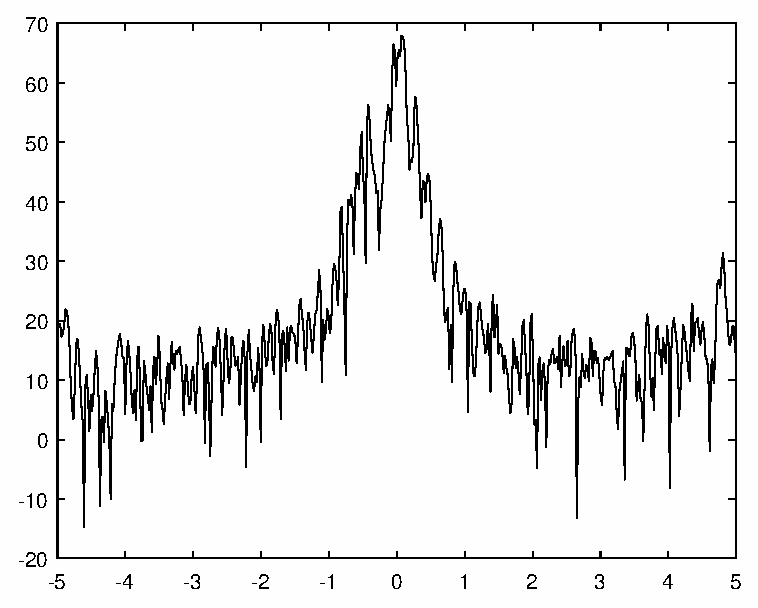
\includegraphics[width=0.4\textwidth]{figures/land}%
		\label{fig:land}}
	\hfil
	\subfloat[海杂波频谱]{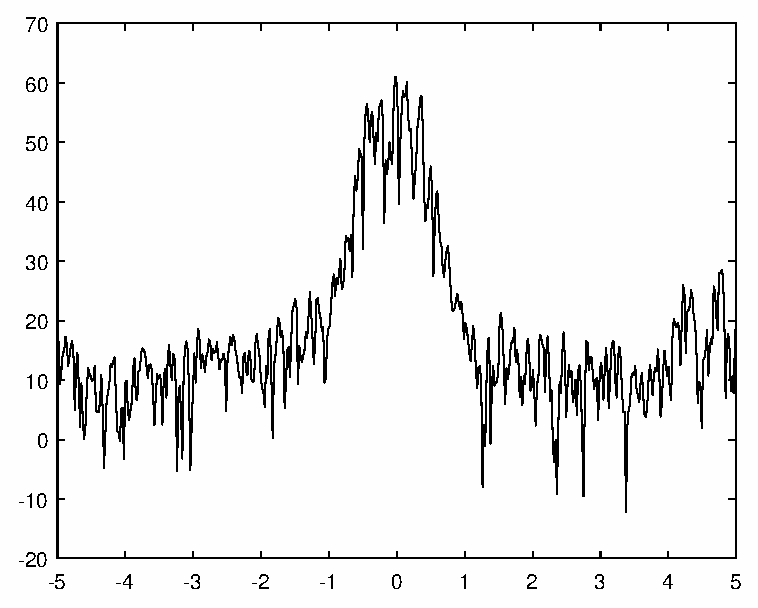
\includegraphics[width=0.4\textwidth]{figures/sea}%
		\label{fig:sea}}
	\caption{These two pictures are not easy to identify. \ref{fig:land} has a little shift, and the Barrage peak pf \ref{fig:sea} cannot distinguish easily.}
	\label{fig:spectrum}
\end{figure}

\subsubsection{数据集分组}
在本章的问题中,当雷达配置发生变化时,我们会获得不同的频率范围和精度频谱数据。例如,一些频谱数据的频率变化范围为-5Hz到5Hz、具有512个相干积累点,而另一些数据的频率变化范围为-10Hz到10Hz、相干积累点数为256个。因此,基于这两个条件,我们将所有数据分为4组:
\begin{itemize}
	\item 组 A: 如图\ref{fig:case25610}所示,具有256个相干积累点数,频率变化范围为-10Hz到10Hz;
	\item 组 B: 如图\ref{fig:case51205}所示,具有512个相干积累点数,频率变化范围为-5Hz到5Hz;
	\item 组 C: 如图\ref{fig:case51210}所示,具有512个相干积累点数,频率变化范围为-10Hz到10Hz;
	\item 组 D: 如图\ref{fig:case102405}所示,具有1024个相干积累点数,频率变化范围为-5Hz到5Hz;
\end{itemize}
我们只选择了上述四个具有典型意义的分组的数据来进行验证,舍弃了其余类型的与他们相似的数据,例如频率变化范围为-10Hz到10Hz的具有512个相干积累点的数据,这与组B的数据基本相同。
\begin{figure*}[!t]
	\centering
	\subfloat[组 A]{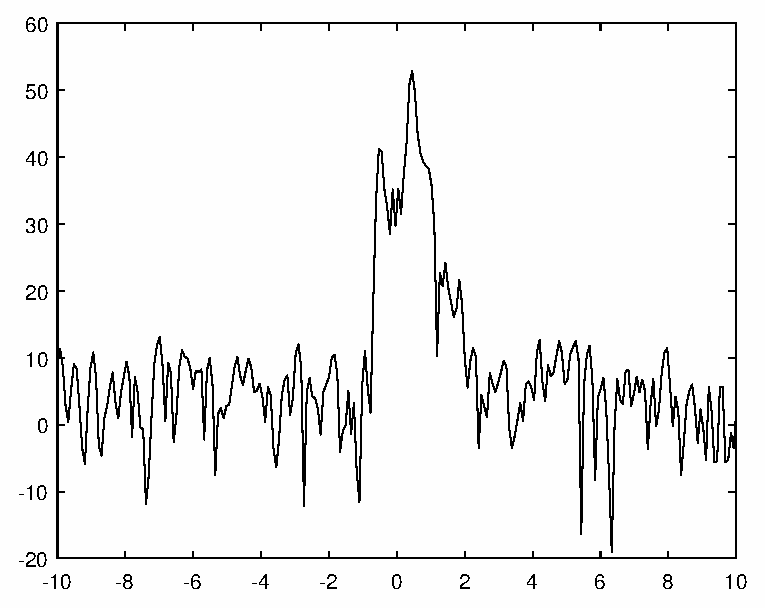
\includegraphics[width=0.4\textwidth]{figures/group256_10}%
		\label{fig:case25610}}
	\hfil
	\subfloat[组 B]{\includegraphics[width=0.4\textwidth]{figures/group512_5}%
		\label{fig:case51205}}
	\centering
	\subfloat[组 C]{\includegraphics[width=0.4\textwidth]{figures/group512_10}%
		\label{fig:case51210}}
	\hfil
	\subfloat[组 D]{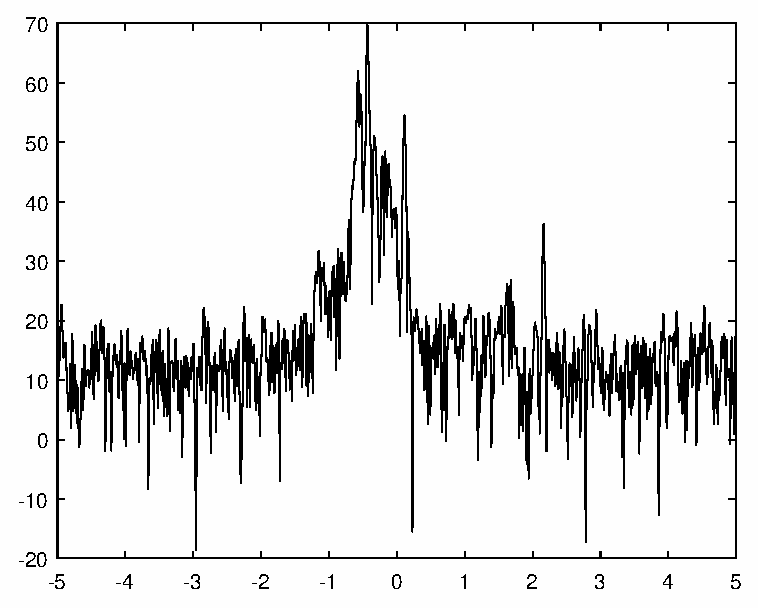
\includegraphics[width=0.4\textwidth]{figures/group1024_5}%
		\label{fig:case102405}}
	\caption{不同组数据的频谱对比示意图}
	\label{fig:group}
\end{figure*}
\subsection{算法实现}
\textcolor{red}{对其余两个算法的介绍}
我们将我们的算法与传统的单特征识别算法和SVM算法进行对比。选择SVM的地海杂波的三个特征是:
\begin{itemize}
	\item 最大后向散射幅值
	\item 频谱中最大与次大幅值频率之差
	\item 频谱中最大与次大幅值幅度之差
\end{itemize}
为了确保我们有足够的数据来训练和测试我们的算法,我们选取了不同的雷达工作条件、天气、时间的多组数据(每组约有20000个频谱数据)。我们随机选择其中$70\%$的数据作为训练数据,$20\%$作为交叉验证数据,其他数据用作测试数据。

\textcolor{red}{测评计算公式叙述}

\subsection{仿真验证}
为了验证我们的深度卷积网络的泛化能力,我们利用了四组数据测试了我们的方法,其不同组数据的损失函数如图\ref{fig:group_results}所示,结果表明我们的算法可以在不同的数据集组中获得良好的结果。虽然,对于相同的神经网络结构,第一个数据集需要最多的迭代次数才能收敛,这是因为当频率和相干累计点的比例变小时信息或者说特征也随之减少,故需要较多的迭代次数。
\begin{figure}[!t]
	\centering
	\includegraphics[width=\textwidth]{figures/group_results}
	\caption{不同数据集损失函数对比图。}
	\label{fig:group_results}
\end{figure}
正如上面描述的,还有另外两种常用的算法来做地海杂波的识别。我们利用实际数据进行实验来对三种算法进行了对比。实验结果如表\ref{tab:methods}所示,可以明显的看到,我们的算法在识别正确率和匹配准确率均为最优。并且,我们可以发现SVM和基准方法都匹配到了错误的区域。\textcolor{red}{此外,当通过整个世界地图找到最大的匹配率时,三种方法与其配对地图在一段时间内的交配率似乎有所不同。}

\textcolor{red}{添加对于三个判断结果参数的设计}
\begin{table}[!t]
	\renewcommand{\arraystretch}{1.3}
	\caption{三种算法识别正确率与匹配正确率计算.}
	\label{tab:methods}
	\centering
	\begin{tabular}{c|ccc}
		\hline
		& 我们的算法 & 支持向量机 & 单阈值算法 \\
		\hline
		识别正确率 & 99.69\% & 92.44\% & 81.85\% \\
		\hline
		最大匹配正确率 & 88.99\% & 22.77\% & 23.48\% \\
		\hline
		匹配正确率 & 88.99\% & 81.31\% & 88.21\% \\
		\hline
	\end{tabular}
\end{table}

图\ref{fig:sizes}展示的是在样本集大小不同的情况下,我们的算法与基准算法的平均分类准确率的对比图。由于基准方法仅使用根据先验知识得到的阈值,因此随数据集增长其识别准确度变化不大,而我们的深度卷积神经网络的算法随着数据集内样本数量的增加,准确度有着显著提升。
\begin{figure}[!t]
	\centering
	\includegraphics[width=\textwidth]{figures/sizes}
	\caption{不同数量数据集的分类准确度对比曲线图}
	\label{fig:sizes}
\end{figure}

众所周知,卷积神经网络的参数对于最终分类识别的准确率起着重要的作用。因此,我们需要对参数的选择进行一些分析。首先,我们分析在批大小(Batch Size)和迭代次数变化时,验证集数据的分类准确度。如图\ref{fig:epoch}所示,我们可以发现识别准确度随着迭代次数的增加而增长。而当批长度变大时,收敛速度加快。
\begin{figure}[!t]
	\centering
	\includegraphics[width=\textwidth]{figures/epoch}
	\caption{不同批长度下,分类准确度与迭代次数曲线图}
	\label{fig:epoch}
\end{figure}

融合预处理参数设计由于滑窗算法的很重要的一个参数就是窗长,针对于本问题主要考虑到电离层会发生变化,过长的窗长对无法及时的响应电离层的变化,影响识别准确率以及地图匹配精度。为了取得一个合适的窗长,我们首先利用不同窗长平均融合后的数据进行测试,得到图 20的结果,该结果也证明了在窗长过长时候,准确率会下降的结论,当窗长过大时准确率会降到比窗长为1时还要低。 图 23 不同窗长识别结果对比图为了进一步比较权重的变化对于识别结果的影响,我们设窗长为 ,样本 的权重为 ,则有融合后的样本为 ,当取权重为 时,得到下面结果,故根据实验结果,本课题最终选择窗长长度为3 图 24 更改权重后不同窗长识别结果对比4.2目标定位精度修正验证由于缺乏实际的 变换相关的航迹信息,故无法对定位精度修正系数进行一个很好的验证。这里我们采用地图变换的过程来进行辅助验证。其基本流程与目标的定位精度修正类似。首先将整个匹配地图划分为很多小的匹配区域,然后对于每个匹配区域分别进行修正系数计算。

如前面所描述的,我们利用融合的方法来减少由于某一帧数据中某距离方位单元由于出现的随机噪声对于我们识别结果的影响。图\ref{fig:window}显示匹配率随着窗口长度的增加首先提高,然后减小。这是因为当窗口过长时,由于天波雷达的采样周期较长,这个期间内,雷达的频谱可能已经出现了一定程度的变化,这回影响最终的识别结果。
\begin{figure}[!t]
	\centering
	\includegraphics[width=\textwidth]{figures/window}
	\caption{The matching rate against fusion window length.}
	\label{fig:window}
\end{figure}
为了找出区分识别结果中海洋与陆地的最佳阈值,我们使用不同的概率阈值计算相同测试数据的正确率。图\ref{fig:threshold}显示,\textcolor{red}{随着阈值越大,增长速度越慢,速率越快}。另一方面,当阈值仅为$0.01$时,识别率仍高于$0.86$。这说明我们的方法的分类结果的概率值均处于较高的水平,如\ref{fig:prob}所示。
\begin{figure}[!t]
	\centering
	\includegraphics[width=\textwidth]{figures/threashold}
	\caption{识别率与概率阈值曲线图.}
	\label{fig:threshold}
\end{figure}
\begin{figure}[!t]
	\centering
	\includegraphics[width=\textwidth]{figures/prob}
	\caption{不同帧数据识别结果概率值}
	\label{fig:prob}
\end{figure}
%\begin{itemize}
%	\item different window and no window
%	\item figures of loss function with time
%	\item dropout changes
%	\item probability threshold changes
%
%	\item fusion and not fusion
%\end{itemize}
\subsection{特征可视化}
\textcolor{red}{该部分需要添加详细的内容}

识别结果的理论分析上面利用大量的测试数据的识别结果以及地图匹配结果对于算法进行了验证,这里我们通过理论分析,验证了算法的合理性。通过计算当输入数据的某个数据点发生变化时输出梯度的变化,得到每一个数据点对于输出梯度的影响,从而得到该频谱数据关注度图。图\ref{fig:visfeature}中红色圆圈部分表示主要利用的特征所在多普勒频率,可以很直观地看出,对于下图这样的海杂波布拉格峰附近频点的数据被关注比较多,另一方面同时兼顾了其余频点的特征,提高了识别准确率。 

卷积神经网络方法有一个问题是其为一个黑盒操作,我们无法直观地看到其用于分类的特征。因此,为了在理论上对于我们算法的有效性进行分析。在本节中,我们使用基于梯度变化的可视化方法,其思想为利用我们已经训练好的模型展示对于其最终判断测试结果为正或者为负主要利用的频谱特征点。我们定义频谱数据序列为$ S = \{s_1, s_2, .., s_n\} $,其中$n$是频谱序列中的点数,设输出概率为$p(S)$。那么,我们可以得到式\ref{equ:ps}:
\begin{equation}
p(S) = w^TS+b,
\label{equ:ps}
\end{equation}
其中$ w $和$ b $分别是我们的模型的权重和偏差。实际上,这里的权重$ w $表示对应点的重要性。在我们的模型中,类概率函数$p(S)$是高度非线性函数,这里使用泰勒方法近似$p(S)$。为了简化计算,我们使用一阶泰勒展开:
\begin{equation}
w = \frac{\partial{p}}{\partial{S}}{\mid}_{s_i}
\label{equ:w}
\end{equation}

\textcolor{red}{因此,我们以通过反向传播计算得到$ w $的方程式\ref{equ:w}(todo:详细描述)。图\ref{fig:vis}显示,特征点主要集中在我们预期的数据上。}
\begin{figure}[!t]
	\centering
	\includegraphics[width=\textwidth]{figures/heatmap.pdf}
	\caption{特征重要程度热力图。}
	\label{fig:vis}
\end{figure}
\begin{figure}[!t]
	\centering
	\includegraphics[width=\textwidth]{figures/heatmap.pdf}
	\caption{某距离方位单元海杂波频谱数据关注度图
	。}
	\label{fig:visfeature}
\end{figure}
\section{小结}
在本章中,我们提出了基于卷积神经网络天波雷达地海杂波识别的新算法。其主要克服了传统的阈值识别方法或支持向量机算法根据经验从频谱数据中提取特征,导致操作复杂度高,分类精度低的缺点。同时,我们将我们的算法与传统算法和支持向量机算法进行了对比。实验结果表明,我们的方法在地海杂波识别问题上更加有效以及抗干扰性能更强。在更高精度的识别结果的帮助下,我们可以得到更加精确的修正系数,可以为目标检测和跟踪问题提供非常大的帮助。
% !Mode:: "TeX:UTF-8"

\chapter{基于深度嵌入卷积聚类方法的地海杂波无监督分类}
\label{sec:decc}
\section{引言}
由于天波雷达地海杂波频谱数据量大,进行人工标定的成本十分昂贵,且当雷达工作频率变化导致数据的相干积累点数变化时需要重新标定数据对网络进行训练。无监督学习(又称聚类)算法是解决该问题的一个很好的思路,但是传统的聚类算法的性能受数据维数以及样本数据量的影响,会产生维数灾难的问题。为了克服这个困难,研究者一般选择将高维度的数据映射到低维,然后将嵌入数据聚类到这个新的子空间中\ucite{roth2004feature}的方法,该方法分为特征学习和聚类这两个割裂的阶段,影响了最终的聚类精度。

本章提出了一种新的联合解决共同完成特征学习和聚类的算法,深度嵌入卷积聚类方法(Deep Embedding Convolution Clustering, DECC)。通过利用卷积自编码器进行特征提取,可以充分挖掘数据的局部信息,设计了新的损失函数用于同时更新网络和聚类中心参数。
% 聚类方法如今已经在各个领域得到了广泛应用
% 对数据集规模较大的情形,有一些研究只选择数据集的一个子集来加速聚类过程\ucite{shinnou2008spectral}。
% 为了解决计算复杂度的问题,以往的研究往往首先
% 这类算法可以分为两个阶段:特征学习和聚类,其主要思想是向目标函数中添加表征稀疏性或者是图形约束的先验知识进行训练学习\ucite{tian2014learning}。

% 特征学习指的是一类试图利用一组通常稀疏的特征向量来描述一个数据集的学习方法。
% 在实践中,有很多不同的算法可以进行特征学习,包括自编码器、高斯混合模型(Gaussian Mixture Model, GMM)和受限玻尔兹曼机。
% 这些方法主要学习一个近似局部滤波器字典\ucite{coates2011analysis},例如用于自然图像的Gabor类边缘滤波器或者用于MNIST数字数据集的书写笔划。

本章安排如下: \ref{sec:cae}节对卷积自编码网络进行了介绍,\ref{sec:decc_method}节构建了本章利用的深度嵌入卷积聚类器,通过利用卷积自编码器对输入地海杂波进行重构,然后利用本章提出的聚类损失函数进行训练,最终获得聚类结果,\ref{sec:decc_experiment}节利用实际数据对本章提出的算法性能进行了分析讨论,\ref{sec:decc_summary}节进行本章总结。

\section{卷积自编码网络}
\label{sec:cae}
\subsection{自编码器}

自编码器是一种利用隐层重构输入的神经网络。其模型如图\ref{fig:ae}所示,它由编码器(Encoder)和解码器(Decoder)两部分组成,本质上是对输入信号的某种变换。
\begin{figure}[hbt]
	\centering
	\includegraphics[width=9cm]{figures/AE/ae}
	\caption{自编码器模型}
	\label{fig:ae}
\end{figure}
对一组具有$N$个输入向量的给定输入数据集,
编码器将第$i$个输入信号$x^{(i)}\in\mathbb{R}^{d_x}$编码到某个隐层的表示$h^{(j)}\in\mathbb{R}^{d_h}$,$d_x$和$d_h$分别为输入表示和隐层表示的维数,然后解码器再将$h^{(j)}$解码为输出$x'^{(i)}\in\mathbb{R}^{d_x}$。通过最小化$x^{(i)}$与$x'^{(i)}$之间的差距,可以训练得到一个用来重构输入特征的映射。
编码和解码公式如下:
\begin{align}
	h^{(j)}_n &= f(b_n+\sum_{m=1}^{d_x}w_{mn}x^{(i)}_m), \\
	x'^{(i)}_m &= f(b'_m+\sum_{n=1}^{d_h}w'_{mn}h^{(j)}_n),
\end{align}
其中,$f$是激活函数函数,${W}=[w_{mn}]$和${W}'=[w'_{mn}]$分别为编码器和解码器的权重矩阵,${b}=[b_n]$和${b'}=[b'_m]$分别为编码器和解码器的偏置向量。

在此基础上,国内外广大学者对自编码器进行了各种改进,提出了可以学习输入空间中扰动不变的特征的压缩自编码器\ucite{rifai2011contractive}、
利用高效的变分方法进行训练和生成推理的变分自编码器\ucite{kingma2013auto}
以及可以基于连续的数据流在运行中添加或合并隐层单元的在线增量自编码器\ucite{zhou2012online}。

\subsection{卷积自编码器}
传统的自编码网络只有一个隐层,只能学习出一种特征变化,于是Bengio\ucite{bengio2007greedy}等人在2007年的仿照stacked RBM构成的DBN,提出堆栈自编码器(Stacked Autoencoders, SAE),为非监督学习在深度网络的应用又增加了一种重要的思路方法。
堆栈自编码器模型可以参看图\ref{fig:sae},其通过逐层非监督学习的预训练,也即逐层初始化(Layer-wise Pre-training),来初始化深度网络的参数,替代传统的随机初始化的方法。预训练完毕后,利用训练参数,再进行监督学习训练。
\begin{figure}[hbt]
	\centering
	\includegraphics[width=9cm]{figures/AE/sae}
	\caption{堆栈自编码器模型}
	\label{fig:sae}
\end{figure}

全连接自编码器和深度自编码器都忽略了数据的局部结构信息。
这在处理实际大小的输入时不仅是一个问题,而且在参数中引入冗余,迫使每个特征是全局的。
然而,在视觉和对象识别领域最成功的模型\ucite{lowe1999object}均主要利用了在整个输入空间发生重复的局部特征。
基于此,文献\cite{masci2011stacked}提出了一种卷积自编码器(Convolutional Autoencoders, CAE)。
卷积自编码器不同于传统的自编码器,它们的权重在输入向量中的所有位置之间共享,从而可以保持空间局部性。
因此重构结果是隐层局部特征的线性组合。
从结构的角度看,CAE类似于SAE,但是将SAE中的全连接神经网络变为了卷积神经网络。
参考第\ref{sec:network}章\equref{equ:shared_weight},设输入为$x$,第$k$个特征映射的隐层表示则由\equref{equ:cae1}给出:
\begin{equation}
	h^k=f(x*W^k+b^k)
	\label{equ:cae1}
\end{equation}
其中$b^k$是全局共享的偏置,$f$是激活函数,$*$表示卷积操作。
% 为了使得每个滤波器专注于整个输入空间的一种特征,另一方面如果每个数据点一个偏置将引入太多的自由度,所以对每一个隐层使用相同的偏置。
\equref{equ:cae1}生成的隐层表示是输入$x$在低维空间中的编码,
由于自编码器的目标是从所生成的特征映射重构输入$x$,因此需要相应的解码操作。卷积自编码器是完全卷积网络,因此解码操作也是一个卷积操作,一般称为反卷积操作(Deconvolution)或者转置卷积(Transposed Convolution)。

隐层表示$h^k$被用来作为解码器的输入,为了使得解码器的输出和原始的输入数据具有相同的结构,解码器反卷积的超参数由编码器的结构确定,
因此,解码器的重构过程的计算公式为:
\begin{equation}
	x'^k=f(\sum_{k \in H}h^k * \tilde{W}^k + b'^k).
	\label{equ:cae2}
\end{equation}
同样的,每一个输入通道只有一个偏置$b'^k$,$H$表示所有特征图的集合,
$\tilde{W}$ 表示在两个维度上进行翻转操作后的权重。

正如第\ref{sec:network}章介绍,一般的分层网络特别是卷积神经网络,通常引入池化层来获得平移不变性。因此本章的卷积自编码器在编码器阶段添加了池化层,相应的在解码器阶段需要添加上采样来进行处理,如图\ref{fig:unpool}所示。
\begin{figure}[hbt]
	\centering
	\includegraphics[width=13.5cm]{figures/AE/unpool}
	\caption{上采样示意图}
	\label{fig:unpool}
\end{figure}

模型参数$\Theta=\{{W},{b},{b'}\}$通过最小化其损失函数进行求取,一般利用均方误差损失函数(mean squared error, MSE):
\begin{align}
	\mathscr{L} &= \frac{1}{N}\sum_{i=1}^N||x_i-x_i'||_2^2, \label{equ:mse_loss}\\
	\theta^* &= arg\min\limits_{\theta} \mathscr{L}.  \label{equ:mse}
\end{align}
就像标准的神经网络一样,反向传播算法被用来计算相对于参数的误差函数的梯度,则可以得到:
\begin{equation}
	\frac{\partial \mathscr{L}}{\partial W^k}=x * \Delta h ^k+\tilde{h}^k * \Delta x',
\end{equation}
$\Delta h$ 和 $\Delta x'$分别是隐层状态和重构结果的变化量,然后可以使用随机梯度下降(SGD)等基于梯度的优化算法来更新权重。

相比于传统自编码器,卷积自编码器更有利于学习数据的局部结构,避免特征空间的失真。
虽然卷积自编码器的过完备隐层表示使得其学习比标准自编码器更难,但是可以通过添加池化层加强其稀疏性来在一定程度上降低计算量。

\section{深度嵌入卷积聚类方法}
\label{sec:decc_method}
深层嵌入聚类算法\ucite{xie2016unsupervised}提供了一种以无监督的方式同时学习特征表示与聚类的思路,提高了聚类算法的性能和鲁棒性。
但是,该算法用于特征提取的堆栈自编码器需要逐层预训练,然后以端到端训练的方式进行微调。当层次增加时,预训练过程所需时间会急剧增加。此外,堆栈自编码器是建立在全连接网络上,对处理局部信息是无效的。
因此本章在此基础上利用卷积自编码器代替传统的堆栈自编码器并设计了新的损失函数,提出了深度嵌入卷积聚类方法(Deep Embedding Convolution Clustering, DECC)。

\subsection{深度嵌入卷积聚类方法结构}
首先进行问题描述,假设需要将$N$个样本$X=[x_1,\dots,x_N]$聚为$K$个类别,其聚类中心点为$\mu_1,\dots,\mu_K$,其中每一个样本$x_i\in \mathbb{R}^{d_x}$,由于当样本维数增大时会会产生维数灾难的问题,因此需要引入一个嵌入函数$\varphi_W: X \rightarrow Z$,可以将原始样本映射到嵌入子空间$Z=[z_1,\dots,z_N]$,其中$z_i\in \mathbb{R}^{d_z}$的维数远小于原始样本的维数,也即$d_z<<d_x$。
然后,利用K-均值聚类算法,将子空间$Z$进行聚类,得到初始聚类中心${\mu_k}$。

本章利用卷积自编码器作为嵌入函数对原始样本进行降维,其结构如图 \ref{fig:cae} 所示。
通过三次卷积操作充分提取输入样本的特征,同时在所有层添加ReLU激活函数,并且在编码器后以相反的顺序放置反卷积解码器。在编码器与解码器中间添加嵌入层(图\ref{fig:cae}中黄色标记的全连接层),该层的结果被用于进行聚类操作。DECC的结构如图 \ref{fig:decc} 所示。
\begin{figure}[hbt]
	\centering
	\includegraphics[width=13.5cm]{figures/AE/cae}
	\caption{卷积自编码器结构图}
	\label{fig:cae}
\end{figure}

\begin{figure}[hbt]
	\centering
	\includegraphics[width=13.5cm]{figures/AE/decc}
	\caption{深度嵌入卷积自编码器结构图}
	\label{fig:decc}
\end{figure}

\subsection{KL散度聚类方法}
文献\cite{maaten2008visualizing}利用学生t分布来衡量嵌入点$z_i$与聚类中心点$\mu_k$的相似度:
\begin{equation}
p_{ik}=\frac{(1+||z_i-\mu_k||^2/\alpha)^{-\frac{\alpha+1}{2}}}{\sum_{k'}(1+||z_i-\mu_k||^2/\alpha)^{-\frac{\alpha+1}{2}}},
	\label{equ:p}
\end{equation}
其中,$\alpha$为学生t分布的自由度,$p_{ik}$可以看作样本$i$到类别$k$的概率。

为了定义本章的聚类目标函数,可以使用辅助目标变量(auxiliary target variable)$Q$来迭代地改进模型预测。首先用Kullback-Leibler(KL)散度来减小模型预测$P$和目标分布$Q$之间的距离。
\begin{equation}
	\mathscr{L}_{kld}=KL(Q||P)=\frac{1}{N}\sum_{i=1}^{N}\sum_{k=1}^{K}q_{ik}\log{\frac{q_{ik}}{p_{ik}}},
	\label{equ:kldfirst}
\end{equation}
根据文献\cite{xie2016unsupervised},目标分布$Q$的定义如下:
\begin{equation}
	q_{ik}=\frac{p_{ik}^2/f_k}{\sum_k(p_{ik}^2/f_k)},
	\label{equ:traget_distribution}
\end{equation}
其中$f_k$的定义为
\begin{equation}
	f_k=\sum_iq_{ik}
\end{equation}

\equref{equ:mse}给出了自编码器重构的损失函数,故最终的损失函数为:
\begin{equation}
	\mathscr{L}=\mathscr{L}_{mse}+\beta \mathscr{L}_{kld},
	\label{equ:l_last}
\end{equation}
其中,$\beta > 0$为调节两部分损失函数权重的参数。

\subsection{学习算法}
本章利用随机梯度下降和反向传播对\equref{equ:l_last}中的损失函数进行学习。根据上一节的描述可知,总共有三类参数需要学习:卷积自编码器的权重、聚类中心以及目标分布$Q$。
\subsubsection{更新卷积自编码器的权重和聚类中心}
对一个给定的目标分布$Q$,那么聚类损失$\mathscr{L}_{kld}$相对于嵌入点$z_i$和聚类中心点$\mu_k$的梯度计算公式如下:
\begin{align}
	\frac{\partial \mathscr{L}_{kld}}{\partial z_i} &= 2\sum_{k=1}^K(1+||z_i-\mu_k||^2)^{-1}(q_{ik}-p_{ik})(z_i-\mu_k), \\
	\frac{\partial \mathscr{L}_{kld}}{\partial \mu_k} &= 2\sum_{i=1}^N(1+||z_i-\mu_k||^2)^{-1}(p_{ik}-q_{ik})(z_i-\mu_k). \\
\end{align}
那么对于一个小的批次$m$和学习率$\lambda$,$\mu_k$的更新为:
\begin{equation}
	\mu_k=\mu_k-\frac{\lambda}{m}\sum_{i=1}^m{\frac{\partial \mathscr{L}_{kld}}{\partial \mu_k}}.
\end{equation}
编码器的权重更新为:
\begin{equation}
	W=W-\frac{\lambda}{m}\sum_{i=1}^m(\frac{\partial \mathscr{L}_{mse}}{\partial W} + \beta \frac{\partial \mathscr{L}_{kld}}{\partial W}).
	\label{equ:encoder_update}
\end{equation}
解码器的权重更新为:
\begin{equation}
	W'=W'-\frac{\lambda}{m}\sum_{i=1}^m{\frac{\partial \mathscr{L}_{mse}}{\partial W'}}.
\end{equation}
\subsubsection{更新目标分布}
根据\equref{equ:traget_distribution}可知,目标分布$Q$依赖于先验的软指派(soft assignment)$P$。因此,为了提升结果的鲁棒性,本章利用全部嵌入点每隔$T$次迭代对目标分布进行更新,其更新主要利用\equref{equ:p}和\equref{equ:traget_distribution}。并且每次完成更新后,重新计算样本$x_i$的指派:
\begin{equation}
	s_i=arg \max \limits_k p_{ik}
	\label{equ:assign}
\end{equation}
当相邻两次更新的指派变化小于一个阈值$\delta$时,停止迭代,那么则可以得到整个算法流程图。
% \\[420pt]
\begin{algorithm}[H]
	\caption{DECC 算法学习过程}
	\begin{algorithmic}[1] %每行显示行号
		\Require 训练样本$X$,聚类结果个数$K$,最大迭代次数$iter_{max}$,目标分布更新间隔$T$,初始目标参数$\theta$,学习率$\eta$
		\Ensure 卷积自编码器编码器的权重$W$和解码器的权重$W'$,聚类中心$\mu$,指派标签$s$
		\State 初始化迭代次数$iter=1$
		\State 只利用重构损失函数对卷积自编码器进行训练,获得初始权重$W$和$W'$
		\State 利用K-均值聚类算法获得初始聚类中心$\mu$
		\While{$iter < iter_{max}$}
			\If{iter mod T = 0}
				\State 计算所有嵌入点 $z_i=\varphi_W(x_i),i=1,\dots,N$
				\State 将\equref{equ:p}代入\equref{equ:traget_distribution}更新目标分布 $Q$
				\State 保存上一次指派$s_{last}=s$
				\State 计算新的指派 $s_i=arg \max \limits_k p_{ik}, i= 1,\dots,N$
				\If{$sum(s_{last} \neq s) / N < \delta $}
					\State 停止学习
				\EndIf
			\EndIf
			\State 从训练集中获取$m$ 个采样样本 $\{x^{(1)},\dots,x^{(m)}\}$ ,其中$m$ 为批处理中一批样本的个数。
			\State 更新聚类中心$\mu_k=\mu_k-\frac{\lambda}{m}\sum_{i=1}^m{\frac{\partial \mathscr{L}_{kld}}{\partial \mu_k}}$
			\State 更新编码器权重 $W=W-\frac{\lambda}{m}\sum_{i=1}^m(\frac{\partial \mathscr{L}_{mse}}{\partial W} + \beta \frac{\partial \mathscr{L}_{kld}}{\partial W})$
			\State 更新解码器权重 $W'=W'-\frac{\lambda}{m}\sum_{i=1}^m{\frac{\partial \mathscr{L}_{mse}}{\partial W'}}$
		\EndWhile
	\end{algorithmic}
\end{algorithm}
\section{仿真验证}
\label{sec:decc_experiment}
% \subsection{算法设置}
本章利用第\ref{sec:othr}章中组C的训练数据用于本章的实验,考虑到地海杂波在时间与空间上的连续性,本章选取了相邻3帧,相邻9个单元共27个单元的杂波信号将其进行组合,并进行随机重排复制得到一个$128\times 128$的二维数据,其示意图参看图 \ref{fig:unsurpvised_data}。
\begin{figure}[hbt]
	\centering
	\includegraphics[width=6.67cm]{figures/AE/unsurpvised_data}
	\caption{输入样本示意图}
	\label{fig:unsurpvised_data}
\end{figure}

本章根据图\ref{fig:cae}设计的卷积自编码器进行特征的降维,该部分进行30次迭代,学习方法为Adam,嵌入层为10维,也即利用10维的特征向量对原始输入信号进行表示。
然后根据此特征向量,随机进行20次K-均值算法,然后从中选取最优结果作为起始的聚类中心点,此也作为本章的一个对比算法。损失函数的权重系数$\beta = 0.1$,学生t分布的自由度$\alpha = 1$。
最终的优化问题通过小批量随机梯度下降和反向传播得到有效解决,其中批长度为256,学习率为0.01。

% \subsection{仿真结果分析}
本章对比了不同算法的无监督聚类精度(ACC)、归一化信息(Normalized Mutual Information, NMI)和调整兰德指数(Adjusted Rand Index, ARI),来比较不同算法的聚类结果的准确率、聚类结果与真实情况的相似程度及每个类内的纯度等信息,实验结果如表\ref{tab:uns}所示。
实验结果证明本章提出的利用深度嵌入卷积算法的正确度相比于K-均值算法有了显著的提高,而添加了重构损失函数后的结果又有了进一步的提高。但是由于卷积运算的计算量比较大以及多个损失函数共同作用导致聚类收敛迭代次数要大于仅利用全连接网络的DEC算法。DECC与DEC的聚类收敛结果的对比,如图\ref{fig:unsurpvised_acc}和\ref{fig:unsurpvised_loss}所示,可以发现DEC算法的收敛速度很快,但是精度不如DECC算法。
\begin{table}[hbt]
	\renewcommand{\arraystretch}{1.3}
	\caption{无监督聚类精度对比表}
	\label{tab:uns}
	\centering\sWuhao
	\begin{tabularx}{\textwidth}{>{\centering\arraybackslash}X>{\centering\arraybackslash}X>{\centering\arraybackslash}X>{\centering\arraybackslash}X>{\centering\arraybackslash}X}
		\toprule
		 方法 & 无监督聚类精度 & 归一化互信息 & 调整兰德指数  \\
		 \midrule
		DEC & $94.88\%$ & 0.73 & 0.81 \\
		CAE + K-均值 & $88.68$ & 0.58 & 0.60  \\
		DECC($\beta=0$) & $95.63\%$ & 0.78 & 0.83 \\
		DECC & $97.85\%$ & 0.86 & 0.92 \\
		 \bottomrule
	\end{tabularx}
\end{table}

\begin{figure}[hbt]
	\centering
	\begin{minipage}{7cm}
		\includegraphics[width=6.67cm]{figures/ae/unsurpvised_acc}
    \caption{DECC与DEC聚类精度对比图}
    \label{fig:unsurpvised_acc}

	\end{minipage}
	\hspace{10pt}
	\begin{minipage}{7cm}
		\includegraphics[width=6.67cm]{figures/ae/unsurpvised_loss}
    \caption{DECC与DEC损失函数对比图}
    \label{fig:unsurpvised_loss}

	\end{minipage}

\end{figure}

\section{小结}
\label{sec:decc_summary}
本章结合卷积神经网络与自编码器提出了深度嵌入卷积聚类方法,利用卷积自编码器进行特征提取使得数据的局部信息得以保留,并在损失函数中将KL散度与重构损失两部分结合有效提高了聚类精度。
虽然与有监督学习算法相比,本章的算法精度仍需进一步提高,但是无监督学习的特性克服了大量数据进行标记的成本过高以及部分数据难以人工准确标记的问题。
% 本章的主要贡献如下:
% \begin{itemize}
% 	\item 本章设计了可以以端到端方式训练的卷积自编码器来从未标记的数据中学习特征。通过在地海杂波数据中包含空间、时间信息,通过添加卷积层、卷积转置层和全连接层,设计了好于传统堆栈自编码器的卷积自编码器。
% 	\item 本章提出了深度嵌入卷积聚类算法来自动聚类地海杂波,DECC利用了卷积自编码器提取局部特征的优势。
% 	\item 利用天波超视距雷达的实际地海杂波数据进行了实验,结果验证了深度嵌入卷积聚类算法的有效性。
% \end{itemize}

\chapter{基于深度学习的辐射源识别}
\label{sec:sei}
% TODO:增加内容与仿真!!!
% 对比利用不同的,添加具体参数的设置。


% 可以考虑进行未经过模糊函数处理和处理之后的对比

% 不同卷积核  学习率  不同卷积核个数
% 层数 节点数等
% 不同训练方法
% 多类别的分类结果图可以参考
% 不同数据的各自的图

\section{引言}
辐射源识别算法需要在无法收集大量数据的前提下正确的对于目标进行分类同时准确区分出已知目标和未知目。
与传统利用已知类别的样本进行训练测试的机器学习算法不同,本站的问题是在Open Set的背景下,需要考虑输入未知分类样本的情况。
由于在复杂电磁环境下传统的辐射源个体识别面临识别能力差和无法识别未知目标等问题与挑战,因此需要寻找一种新的方法解决该问题。

本章综合雷达信号处理、深度学习等多学科理论,通过对实际数据的分析,结合深度卷积神经网络与支持向量机方法,以雷达信号的模糊函数切片作为训练样本的特征向量,构建了一个可以对未知分类进行辨识的分类器。最后,利用实际数据进行验证,证明本章提出的分类器具有很高的准确性。

本章安排如下: \ref{sec:sei_data}节对辐射源信号进行了分析,并对其进行预处理,求取其模糊函数切片,\ref{sec:sei_method}节构建了本章的Open Set 分类器,详细地阐述了深度卷积神经网络这个主分类器与支持向量机Meta-Recognition的设计过程,\ref{sec:sei_experiment}节利用实际数据对于分类器已知分类识别和未知分类辨别的性能进行了验证,\ref{sec:sei_summary}节进行本章总结。

\section{辐射源信号分析}
\label{sec:sei_data}
对辐射源信号的分析处理,本章主要考虑两方面:信号预处理、特征提取优化。
本章所获得的信号为雷达辐射源的I/Q两路数据,这是一种在雷达信号处理领域常见的用来描述信号的方法。其中I表示In-Phase,即同相;Q表示Quadrature,即正交,与I相位之差为90度。
设需要表示的信号的峰值幅度为$A$、相位角为$\phi$,则有:
\begin{equation}
	I = A\cos{\phi}
	\label{equ:i}
\end{equation}
\begin{equation}
	Q = A\sin{\phi}
	\label{equ:q}
\end{equation}
也即,可以利用\equref{equ:signal}表示信号:
\begin{equation}
	Ae^{i\phi}=A(\cos(\phi) + i\sin(\phi))=I+Qi
	\label{equ:signal}
\end{equation}
从而可以根据\equref{equ:i}和\equref{equ:q}利用I/Q数据求取信号的峰值幅度和相位角:
\begin{equation}
	A=\sqrt{I^2+Q^2}
\end{equation}
\begin{equation}
	\phi=tan^{-1}(Q/I)
\end{equation}
在完成信号形式的转换后,首先需要对信号进行初步的预处理,剔除无用和错误的数据。
在特征提取优化方面,合理的特征是分类识别的基础。由于存在相同型号的辐射源,利用简单的参数特征无法很好的完成辐射源的个体识别,但是在实际中辐射源自身存在相位噪声以及各类杂散输出,此部分特征可以用来区分出型号、参数均相同的辐射源,因此需要选取一种可以提取雷达辐射源这种无意调制产生的信号脉内细微特征的方法。
模糊函数不仅能描述辐射源信号的分辨特性与模糊度,还能描述由雷达辐射源信号所决定的测量精度、杂波抑制特性等,通过模糊函数在时延和频偏这两个维度上的变换,可以多角度的刻画出无意调制对于发射信号的影响,最终选取了利用雷达模糊函数挖掘辐射源的特征。
\subsection{模糊函数}
对于信号$x(t)$,其瞬时自相关函数为$R_x(t,\tau)=x(t+\tau/2)x^{*}(t-\tau/2)$,其中$\tau$为时延,模糊函数的定义为,
\begin{equation}
A(\tau,\nu) = \int_{-\infty}^{+\infty}R_x(t,\tau)e^{j2\pi\nu t}dt
\label{equ:defineaf}
\end{equation}
即$R_x(t,\tau)$关于时间$t$的傅里叶反变换。

为了方便在数字信号中使用,\equref{equ:defineaf}可以经过变换等价于下面的形式:
\begin{equation}
A(\tau,\nu) = \int_{0}^{\tau}x(t)x^{*}(t+\tau)e^{j2\pi\nu t}dt
\label{equ:afcon}
\end{equation}
对信号均匀采样,即对接收信号和参考信号离散化后,\equref{equ:afcon}可以表示为:
\begin{equation}
A(\tau_l,\nu_m) = A(l, m) = \sum_{n = 0}^{N-1}x(n)x^{*}(n+l)e^{\frac{j2\pi m n}{N}}
\end{equation}
其中,$\tau_l=l/f_s$、$\nu_m=mf_s/N$。

此处以一个简单的单载频矩形脉冲信号来展示模糊函数特征提取的作用,图\ref{fig:danpinmaichong}为模糊函数图,可以发现模糊函数存在一定的冗余,其主要变化均处于0时偏和0频偏附近。
为了减小计算量,本章在频偏为0附近取不同时间延迟的切片作为信号特征,即可以有效地提取信号的相位噪声和杂散输出等个体特征,并且此处受噪声的干扰较小,更加稳定,图 \ref{fig:qiepian}即为在频偏为0处的单载频矩形脉冲信号模糊函数切片。

\begin{figure}[hbt]
	\centering
	\begin{minipage}[b][][b]{7cm}
		\centering
		\includegraphics[width=6.67cm]{figures/emitter/danpinmaichong}
		\caption{单载频矩形脉冲信号模糊函数图}
		\label{fig:danpinmaichong}
	\end{minipage}
	\hspace{10pt}
	\begin{minipage}[b][][b]{7cm}
		\centering
		\includegraphics[width=6.67cm]{figures/emitter/qiepian}
		\caption{单载频矩形脉冲信号模糊函数切片}
		\label{fig:qiepian}
	\end{minipage}

\end{figure}

\section{Open Set 分类器设计}
\label{sec:sei_method}
通常的识别或者分类系统仅考虑的是一个闭集分类系统,然而在现实世界中,这种分类系统会遇到很大的问题。由于其最基本的假设是所有的类别均为先验已知,那么就会出现问题,例如在训练样本中不存在类别的样本就会被错误的分到某个类别中去。这种在训练过程提供不完整的信息,而在测试时添加未知分类的问题,称作Open Set识别\ucite{scheirer2013toward, jain2014multi}。这个问题还可以描述为需要在测试过程中拒绝未知样本。Open Set目标识别系统必须可以准确的处理下面三种类型的数据类:
\begin{itemize}
	\item 已知的(目标)类,被标记为正训练样本的数据。
	\item 已知的未知(非目标)类,被标记为负训练样本的数据。
	\item 未知的未知(非目标)类,在训练样本中不存在的类别的数据。
\end{itemize}
传统的机器学习算法均是针对闭集数据设计的,随着识别算法应用场景的增多和对精度要求的提高,许多学者开始了对Open Set识别的研究。Simonson\ucite{simonson1998probabilistic}提出了一种称作概率融合(probabilistic fusion, PF)的利用统计的方法来进行Open Set识别,其主要通过合并来自不同数据源的证据得到一个统计测试模型,根据此模型的分布来对于类别进行判断。Scheirer等人\ucite{scheirer2011meta}提出了一种通过分析后验数据得分来进行类型判断的方法。

此部分主要解决的问题是当得到一个新的测试样本,如果该样本不属于已经经过训练的分类,那么传统的神经网络模型会将该样本指派给与其最相似的一个类别,此种情况对一个Open Set识别系统,也即类似于辐射源识别系统这种具有较多尚未经过训练的样本的一个数据集,首先这会导致其识别率下降,另一方面是由于对未知辐射源无法很好的确定,无法很好的完成预警等任务。
目前,学者对该问题的研究主要分为下面两个思路:
\begin{itemize}
	\item 在训练集中添加一个“未知”类别,利用不同的来自非已知类别的数据作为训练样本对该类别进行训练,然后对于所有的输入数据进行类别的识别,对于识别结果为该类别的数据作为未知分类。
	\item 针对多分类使用的softmax函数,可以设立阈值或者对该识别结果进行一个评价(例如与已知类别数据的一个“距离”),通过这种方式分辨出未知分类。
\end{itemize}
第一个思路最大的问题是实际工程中无法得到所有可能的未知类别的样本来进行训练,具有一定的局限性,不适用于本章这个具有大量来自未知分类数据的问题。针对于该问题,本章基于后一个思路设计了一个基于Meta-Recognition的可以识别未知辐射源的深度神经网络。首先是创建一个深度卷积神经网络分类器,该分类器的输出为该训练样本属于各个类别的概率,然后将此类别作为一个输入,输入到一个支持向量机分类器Meta-Recognition中,然后利用该Meta-Recognition判断输入是否为未知分类。
\begin{figure}[hbt]
	\centering
	\includegraphics[width=13.5cm]{figures/emitter/frame_emitter}
	\caption{分类器设计结构图}
\end{figure}

\subsection{深度卷积神经网络分类器设计}
本章根据辐射源信号的实际数据以及其反映出来的特性,设计了一个如图\ref{fig:struct_emitter}所示具有10层的一维卷积神经网络。
该分类器作为主分类器,且Meta-Recognition是以该分类器的输出作为输入,所以该分类器性能的好坏会直接影响到对已知类别的分类和对未知类别的判断。

第一层是输入层,由于模糊函数切片为一个$1 \times 1000$的向量,因此输入层大小是$1 \times 1000$。

第二层是卷积层$C1$,$C1$对输入向量进行一维卷积运算提取特征,卷积运算可以最
大程度的提取原始信号的特征。此处利用了256个大小为$1\times 3$的卷积滤波器,其窗口移动步长为1。

第三层是一个池化层$S2$,$S2$层对上一层$C1$做池化处理,池化的目
的是在保留数据有用信息的同时,尽可能减少数据量。此处采用的是$1\times 2$的最大池化操作。

第四层是一个卷积层 $C3$,$C3$对$S2$的特征进行卷积操作,此处利用了128个大小为$1\times 3$的卷积滤波器。

第五层是一个卷积层 $C4$,其结构与$C3$相同,128个大小为$1\times 3$的卷积滤波器。

第六层是一个池化层 $S5$,其结构与$S2$相同,$1\times 2$的最大池化操作。

第七层是一个卷积层 $C6$,其结构与$C3$相同,128个大小为$1\times 3$的卷积滤波器。

第八层是一个卷积层 $C7$,其结构与$C3$相同,128个大小为$1\times 3$的卷积滤波器。

第九层是一个池化层 $S8$,其结构与$S2$相同,$1\times 2$的最大池化操作。

第十层是输出层,根据不同的类别个数选取相应的输出节点个数,首先将$S8$的特征拉成一个一维向量,然后通过全连接网络与输出层进行连接,通过Softmax激活函数输出最终的结果。

\begin{figure}[hbt]
	\centering
	\includegraphics[width=13.5cm]{figures/emitter/struct_emitter}
	\caption{深度卷积神经网络框架图}
	\label{fig:struct_emitter}
\end{figure}

\subsection{支持向量机 Meta-Recognition 设计}

\subsubsection{支持向量机原理}
支持向量机是一种流行的分类方法,它可以在不需要大量数据的情况下产生良好的结果。对一个二分类问题,设$((x_1,y_1),\dots,(x_n,y_n))$为训练数据集,其中$x_i$为某样本的特征向量,$y_i\in\{-1,+1\}$为该样本的标签。支持向量机的思想为找到一个超平面将这些样本划分为正类(标签为$+1$)和负类(标签为$-1$),并且使得正类和负类之间的距离最大。这个超平面的间隔被定义为正类与负类之间的最近距离。

对于一个线性分类问题,假设所有的数据满足下面的约束:
\begin{equation}
	w\cdot x_i +b \geq + 1 \quad y_i = +1
	\label{equ:constraint1}
\end{equation}
\begin{equation}
	w\cdot x_i +b \leq + 1 \quad y_i = -1
	\label{equ:constraint2}
\end{equation}
其中$w$为超平面的法向量,$\frac{|b|}{||w||}$是从超平面到原点的垂直距离,$||w||$是向量$w$的欧拉范数。将上述两个式子合并得到:
\begin{equation}
	y_i(w\cdot x_i+b)\geq 1 \forall i
	\label{equ:svm}
\end{equation}
\equref{equ:svm} 中的训练样本构成了这个分类平面(图 \ref{fig:hyperplanes} 中的$H_1$与$H_2$)。间隔 $\rho$ 可以通过计算$H_1$与$H_2$的距离得到:
\begin{equation}
	\rho=\frac{|1-b|}{||w||}-\frac{|-1-b|}{||w||}=\frac{2}{||w||}
\end{equation}
\begin{figure}[hbt]
	\centering
	\includegraphics[width=6.67cm]{figures/emitter/svm_hard}
	\caption{标准分类平面,即具有最大间隔的超平面。被圈起来的样本组成了这个超平面,其被称作支持向量。}
	\label{fig:hyperplanes}
\end{figure}
因此求解标准分类超平面的最大间隔的问题,就转变为下面的优化问题。
\begin{equation}
	\min \limits_{w\in \mathcal{H}} \tau(w)=\frac{1}{2}||w||^2\quad s.t. \quad y_i(w\cdot x_i +b) \geq 1 \quad \forall i
	\label{equ:optimization}
\end{equation}

为了使得约束更好表示,可以用拉格朗日优化算法对上式重新描述,
\begin{equation}
	\min \limits_{w,b} L(w,b,\alpha)=\frac{1}{2}||w||^2-\sum_{i=1}^l\alpha_i y_i (x_i w + b) + \sum_{i=1}^l{\alpha_i}
	\label{equ:lagrange}
\end{equation}
其中$\alpha_i \geq 0$为约束条件。

在实际计算过程中,可以通过对偶定义求解优化方程\equref{equ:lagrange},通过最大化方程\equref{equ:lagrange}相对于$\alpha$来求取其相对于$w$和$b$的最小值。利用 Karush-Kuhn-Tucker 条件,则\equref{equ:lagrange}变为下面对偶形式:
\begin{equation}
	\max \limits_{\alpha} L_D=\sum_i{\alpha_i}-\frac{1}{2}\sum_{i,j}\alpha_i\alpha_jy_iy_jx_i\cdot x_j \quad s.t. \quad \forall i
	\left\{
		\begin{aligned}
	   &\sum_i{\alpha_iy_i}=0  \\
	   &\alpha_i \geq 0
	   \end{aligned}
		\right.
\end{equation}
因此,通过求解这个对偶优化问题,可以得到系数$\alpha_i$。其中满足$\alpha_i>0$的解称作支持向量,他们位于标准分类平面$H_1$或者$H_2$上。注意到,仅有$\alpha_i>0$的解影响最终的支持向量的选择。
因此,可以得到决策函数:
\begin{equation}
	f(x)=w^Tx_i+b=\sum_{i=1}^My_i\alpha_i(x_i^Tx)+b
\end{equation}
决策函数的符号取决于预测样本$x$。

此处讨论的情形的一个假设是可以把所有的样本完全分为不同的类别。但是显然在大多数情况下,这种假设是不成立的。另外,这种假设也会导致过拟合现象的出现。因此,文献 \cite{cortes1995support} 提出了软间隔的支持向量机。
其主要思想是,通过引入正的松弛变量$\xi_i$来放宽\equref{equ:constraint1}和\equref{equ:constraint2}的约束。基于此,得到\equref{equ:constraint_soft}

\begin{equation}
	\forall i \quad
	\left\{
	 \begin{aligned}
	&w\cdot x_i + b \geq +1-\xi_i \quad y_i=+1  \\
	&w\cdot x_i + b \leq -1-\xi_i \quad y_i=+1  \\
	&\xi_i \geq 0
	\end{aligned}
	 \right.
	\label{equ:constraint_soft}
\end{equation}
这允许一些样本在边缘内部,甚至在相反类别的情况下进一步交叉(见图\ref{fig:softmargin})。 虽然这种松弛使得支持向量机能够灵活地降低异常值的影响,但是从优化问题求解的角度来看,任意大的松弛变量$\xi_i$可能会导致SVM获得平凡解或次优解。 因此,可以通过使松弛变量成为\equref{equ:optimization}的一部分,来限制松弛度:
\begin{equation}
	\min \limits_{w\in \mathcal{H},\xi\in \mathbb{R}^m} \tau(w,\xi)=\frac{1}{2}||w||^2+C\sum_{i=1}^m {\xi_i}
\end{equation}
\begin{figure}[hbt]
	\centering
	\includegraphics[width=6.67cm]{figures/emitter/svm_soft}
	\caption{软间隔支持向量机}
	\label{fig:softmargin}
\end{figure}
其约束条件为\equref{equ:constraint_soft}。超参数$C>0$是针对于误分类的惩罚系数,该系数需要根据不同的分类任务和数据集进行调整。
将其变为的对偶形式,则有
\begin{equation}
	\max \limits_{\alpha} L_D=\sum_i{\alpha_i}-\frac{1}{2}\sum_{i,j}\alpha_i\alpha_jy_iy_jx_i\cdot x_j \quad s.t. \quad \forall i
	\left\{
		\begin{aligned}
	   &\sum_i{\alpha_iy_i}=0  \\
	   &C \leq \alpha_i \geq 0
	   \end{aligned}
		\right.
	\label{equ:cdotdual}
\end{equation}

目前只是分析了线性支持向量机的问题,为了应对非线性分类问题,引入了核函数的概念。将训练数据通过某函数$\Phi:\mathbb{R}^d\mapsto\mathcal{H}$。经过该变换后,只需要将原来计算$\mathbb{R}^d$的$x_i\cdot x_j$变为计算在$\mathcal{H}$域的向量积$\Phi(x_i)\cdot\Phi(x_j)$。为了降低计算量,可以引入核函数$K$来避免数据$x_i$和$x_j$从$\mathbb{R}^d$映射到$\mathcal{H}$。
\begin{equation}
	K(x_i,x_j)=\Phi(x_i)\cdot\Phi(x_j)
\end{equation}
因此,可以将\equref{equ:cdotdual}变为:
\begin{equation}
	\max \limits_{\alpha} L_D=\sum_i{\alpha_i}-\frac{1}{2}\sum_{i,j}\alpha_i\alpha_jy_iy_j K(x_i,x_j)\quad s.t. \quad \forall i
	\left\{
		\begin{aligned}
	   &\sum_i{\alpha_iy_i}=0  \\
	   &C \leq \alpha_i \geq 0
	   \end{aligned}
		\right.
\end{equation}
常用的核函数有下面几种:
\begin{itemize}
	\item 线性核函数:$K(x,y)=x^Ty+C$
	\item 多项式核函数:$K(x,y)=(x^Ty+C)^d$
	\item RBF 核函数:$K(x,y)=e^{\frac{-||x-y||^2}{2\sigma^2}}$
	\item Sigmoid 核函数:$K(x,y)=\tanh(\alpha x^Ty+C)$
\end{itemize}
\subsubsection{支持向量机设计}
本章利用所有的目标数据和未知目标的数据来作为训练样本对该SVM分类器进行训练,本部分以深度卷积神经网络的输出作为该分类器的输入,利用各类别的概率作为其特征进行训练识别。由于在类别的识别过程中,存在一定的波动性,这个会影响结果是否属于未知类别的分类判断,本章选取来自同一个辐射源的连续10拍的识别结果进行一个平均作为最终的输入。

下面是支持向量机分类器的设计,首先是核函数的选择。核函数将输入空间映射到高维特征空间,最终在高维特征空间中构造出最优分类超平面,从而把平面上本身不好分的非线性数据分开。常用的核函数为线性核函数和径向基核函数( Radial Basis Function, RBF)。在核函数的选择方面,当特征数量很大时一般选用线性核函数,而对本章这种特征数量比较小的问题,一般选择径向基核函数。

具有径向基核的支持向量机具有两个关键参数,惩罚参数$C$的和核参数$\sigma$,这两个参数的取值在很大程度上决定了SVM的性能的优劣。
核参数$\sigma$主要影响样本数据在高维特征空间中分布的复杂程度,即维数。特征子空间的维数越高,那么得到的最优分类超平面就会越复杂。因此只有选择合适的核参数得到合适的特征子空间,才能得到泛化能力良好的SVM分类器。大量的实验数据表明,如果与样本点之间的距离很小,$\sigma \rightarrow 0$;如果与样本点之间的距离很大时,$\sigma \rightarrow \infty$;当$\sigma$很小,径向基核函数支持向量机得到的判别函数差不多是一个常数,出现过拟合现象。当$\sigma$很大时,样本的正确分类率也会比较低。

惩罚参数是影响SVM算法性能的另一个重要因素。它的作用主要是调节特征子空间中SVM模型的置信范围与经验风险的比例,使支持向量机的泛化能力达到最好。特征子空间不同时,最优参数值取值也会不同。惩罚参数与经验误差的惩罚和SVM的复杂度成正比,与经验风险值成反比。因此,选择合适的惩罚参数也是非常重要的。

\section{仿真实验与分析}
\label{sec:sei_experiment}
\subsection{实验环境}

本章利用了来自13架民航飞机的气象雷达辐射源的数据,飞机信息参见表\ref{tab:flight}
\begin{table}[hbt]
	\renewcommand{\arraystretch}{1.3}
	\caption{辐射源信号数据}
	\label{tab:flight}
	\centering\sWuhao
	\begin{tabularx}{\textwidth}{>{\centering\arraybackslash}X>{\centering\arraybackslash}X>{\centering\arraybackslash}X}
		\toprule
		 飞机地址码 & 飞机航班号 & 飞机型号  \\
		 \midrule
		 7BF014 & CCA1416 & Airbus A330 (twin-jet)\\
		 780DB3 & TBA9881 & Airbus A330 (twin-jet) \\
		 780E06 & CSN3438 & Airbus A330 (twin-jet\\
		 780EBB & CES293 & 	Airbus A321 (twin-jet)\\
		 780EBF & CES2342 & Airbus A320 (twin-jet)\\
		 7804F2 & ZH9164 & Airbus A320 (twin-jet)\\
		 7804F4 & CES5856 & Boeing 737\\
		 7806FC & CSN6402 & Airbus A320 (twin-jet)\\
		 7808F0 & CES5373 & Airbus A319 (twin-jet)\\
		 78057F & CCA4103 & Airbus A321 (twin-jet\\
		 780063 & CCA4377 & Airbus A319 (twin-jet)\\
		 780375 & CSC8253 & Airbus A319 (twin-jet)	\\
		 781022 & EU2731 & Airbus A319 (twin-jet)\\
		 \bottomrule
	\end{tabularx}
\end{table}

本章的气象雷达辐射源信号,原始的雷达信号为如图 \ref{fig:IQ} 所示的I/Q信号,
为了更好的捕捉到雷达辐射源回波的特征信息,本章对数据进行了一个变换,利用快速傅里叶变换求取其模糊函数,并做偏移为0附近的一个切片作为输入的特征向量,经过变换后的样本的特征如图\ref{fig:diff_data}所示。
\begin{figure}[hbt]
	\centering
	\begin{minipage}{7cm}
		\centering
		\includegraphics[width=6.67cm]{figures/emitter/IQA}
		\caption{原始I/Q信号}
		\label{fig:IQ}
	\end{minipage}
	\hspace{10pt}
	\begin{minipage}{7cm}
		\centering
		\includegraphics[width=6.67cm]{figures/emitter/diff_data}
		\caption{不同类别样本特征图}
		\label{fig:diff_data}
	\end{minipage}
\end{figure}
由于该变换后,数据之间的差距比较大,本章对数据利用离差标准化(Min-Max Normalization)方法进行归一化,是对原始数据的线性变换,使结果值映射到$[0 , 1]$之间。转换函数如下:
\begin{equation}
x^{*}=\frac{x-x_{min}}{x_{max}-x_{min}}
\end{equation}
其中$x_{max}$为样本数据的最大值,$x_{min}$为样本数据的最小值。

在数据的选择方面,本章从数据中选择出2至8个类别分别进行实验,对于每一个类别,也即每架飞机原始信号为100次雷达扫描周期的信号。
由于深度学习需要大量的数据进行训练学习,而本身数据量偏少,故本章在已有数据的基础上在一定信噪比的前提下,生成部分仿真数据,最终每架飞机均有10000组信号。对于这些信号,本章选择其中的$70\%$作为训练样本,$20\%$用于交叉验证,$10\%$作为测试,同时在测试样本中添加与其等量的来自未训练类别也即未知类别的样本共同作为测试样本用来衡量其未知分类的识别率。
本章采用网格搜索法对SVM参数进行调优,最终选择参数惩罚参数为$C=32$,核参数$\sigma=0.0312$。

\subsection{实验结果分析}

\subsubsection{深度卷积神经网络识别结果}

首先验证深度卷积算法的识别正确率,利用8个类别的数据进行训练和测试,迭代次数为100次,其分类结果如表\ref{tab:cnn_29}所示。从表格中容易看出,每一个单独类别的分类精度都很高。
\begin{table}[hbt]
	\renewcommand{\arraystretch}{1.3}
	\caption{深度卷积神经网络分类结果}
	\label{tab:cnn_29}
	\centering\sWuhao
	\begin{tabular}{ccccccccc}
		\toprule
		 & 类别 A & 类别 B & 类别 C & 类别 D & 类别 E & 类别 F & 类别 G & 类别 H \\
		 \midrule
		 类别 A & 100\% & 0 & 0 & 0 & 0 & 0 & 0 & 0 \\
		 类别 B & 7.42\% & 92.58\% & 0 & 0 & 0.13 & 0 & 0 & 0 \\
		 类别 C & 0 & 0 & 97.83\% & 0 & 0 & 2.17\% & 0 & 0 \\
		 类别 D & 0 & 0 & 3\% & 97\% & 0 & 0 & 0 & 0 \\
		 类别 E & 0 & 0 & 0 & 0 & 100\% & 0 & 0 & 0 \\
		 类别 F & 0 & 0 & 0.08\% & 0 & 0 & 99.92\% & 0 & 0 \\
		 类别 G & 0 & 0 & 1.08\% & 0 & 0 & 0 & 98.92\% & 0 \\
		 类别 H & 1.63\% & 0 & 0 & 0 & 0 & 0.63 & 0 & 98.37\% \\
		\bottomrule
	\end{tabular}
\end{table}

同对迭代次数与识别准确率和损失函数进行了验证,其结果如图 \ref{fig:openset_epoch}、图\ref{fig:diff_loss}和表\ref{tab:cnn_epoch_29}所示,无论是训练样本还是测试样本,其精度与损失函数均很快收敛到比较好的水平,不过相应的学习时间也正比增长,故在实际工程中需要对精度和时间进行衡量选取一个最合适的迭代次数。
\begin{table}[hbt]
	\renewcommand{\arraystretch}{1.3}
	\caption{深度卷积神经网络分类结果}
	\label{tab:cnn_epoch_29}
	\centering\sWuhao
		\begin{tabularx}{\textwidth}{>{\centering\arraybackslash}X>{\centering\arraybackslash}X>{\centering\arraybackslash}X>{\centering\arraybackslash}X}
		\toprule
		迭代次数 & 训练样本学习正确率 & 测试样本学习正确率  &  学习时间(s) \\
		 \midrule
			1 & 0.4670 & 0.5782 & $1.0931\times 10^3$ \\
			2 & 0.7658 & 0.7758 & $2.3572\times 10^3$ \\
			10 & 0.9414 & 0.8102 & $1.1444\times 10^4$ \\
			20 & 0.9709 & 0.9065 & $2.1370\times 10^4$ \\
			40 & 0.9819 & 0.9883 & $4.3181 \times 10^4$ \\
			50 & 0.9839 & 0.9830 & $5.3437 \times 10^4$ \\
			60 & 0.9866 & 0.9746 & $6.4143 \times 10^4$ \\
			70 & 0.9903 & 0.9904 & $7.4849 \times 10^4$ \\
			80 & 0.9904 & 0.9798 & $8.5597 \times 10^4$ \\
			90 & 0.9908 & 0.9872 & $9.6328\times 10^4$ \\
			100 & 0.9902 & 0.9811 & $1.0711 \times 10^5$ \\
		\bottomrule
	\end{tabularx}
\end{table}

\begin{figure}[hbt]
	\centering
	\begin{minipage}{7cm}
		\centering
		\includegraphics[width=6.67cm]{figures/emitter/diff_epoch}
		\caption{迭代次数与识别准确率曲线图}
		\label{fig:openset_epoch}
	\end{minipage}
	\hspace{10pt}
	\begin{minipage}{7cm}
		\centering
		\includegraphics[width=6.67cm]{figures/emitter/diff_loss}
		\caption{迭代次数与损失函数曲线图}
		\label{fig:diff_loss}
	\end{minipage}
\end{figure}
\subsubsection{Open Set 分类器识别结果}

在上述样本的情形下,可以通过选取不同的类别数目,进行实验得到表\ref{tab:nb_classes}的识别结果。易知,随着样本类别数的增加,对于未知分类的识别准确率也随之有了大幅度的增加,而另一方面随着类别的增加,对于每个类别的识别准确率仍然维持在比较高的水平。

\begin{table}[hbt]
	\renewcommand{\arraystretch}{1.3}
	\caption{不同已知类别个数数据识别结果}
	\label{tab:nb_classes}
	\centering\sWuhao
	\begin{tabularx}{\textwidth}{>{\centering\arraybackslash}X>{\centering\arraybackslash}X>{\centering\arraybackslash}X}
		\toprule
		 已知类别数目 & 已知类别识别正确率 & 未知类别分辨正确率 \\
		\midrule
		2 & 99.55\% & 84.32\% \\
		3 & 99.59\% & 93.10\% \\
		4 & 99.00\% & 97.81\% \\
		5 & 99.75\% & 98.42\% \\
		6 & 98.63\% & 98.85\% \\
		7 & 99.28\% & 99.22\% \\
		8 & 97.86\% & 99.14\% \\
		\bottomrule
	\end{tabularx}
\end{table}

\section{小结}
\label{sec:sei_summary}
本章针对复杂电磁环境下辐射源的识别面临的电磁信号干扰大、雷达信号参数相近等问题与挑战,利用深度学习的思想与方法,深入研究辐射源脉内细微特征,设计合适的神经网络结构,并基于民航机载气象雷达数据进行初步验证。本章的主要贡献如下:

(1)本章设计了Meta-Recognition,实现了对辐射源中未知分类的辨别。

% (1)利用深度学习方法进行辐射源识别前沿。虽然已有研究利用神经网络、支持向量机等机器学习算法进行识别,但是仍然需要基于雷达信号的基本参数,没有考虑信号的内部特征参数。

(2)本章采用方法具有较强的抗噪声、抗干扰能力以及较好的鲁棒性。传统方法进行辐射源个体识别前均需进行降噪、多径抑制和分选等复杂的信号预处理工作,这些操作会在一定程度上削弱雷达的个体特征。通过对现有辐射源信号进行分析,深度学习方法利用其脉内细微特征作为训练样本,使得识别准确率有了较大的进步。
% 可以通过大量的样本,智能地判断各特征的权重,通过赋予不同的权重在保留雷达个体特征的情况下,避免干扰的影响。

% !Mode:: "TeX:UTF-8"

\chapter{总结}
\label{sec:paper_summary}
\section{本文的主要贡献}
雷达信号分类一直是雷达领域一个很重要的方面,通过对接受到的信号的分类识别,可以更好的了解战场形势。在电子科技迅猛发展的今天,电磁环境急剧变化,雷达信号分类在军事侦查、目标识别、电子对抗等领域有着广阔的应用前景。
而深度学习方法由于其在识别分类等领域的优势,引起了国内外越来越多学者的重视。本文对雷达信号分类中的天波雷达地海杂波识别和辐射源识别这两个方面进行了研究,通过对雷达信号数据的分析,构建合理的卷积神经网络模型,实现了雷达信号类别的识别,并尝试使用无监督方法进行聚类识别。另一方面,针对辐射源识别过程中存在未知类别的情况,构建了一个支持向量机分类器作为Meta-Recognition对深度卷积神经网络的识别结果进行二次处理,实现了未知分类的辨别。
本文的主要研究成果和最终的结论如下:

本文首先叙述了深度学习的研究现状和发展及与传统神经网络方法相比的优点所在,同时描述了深度学习的几种常用方法和基本结构,研究了深度卷积神经网络的原理和其训练过程。

针对天波雷达中由于电离层的变化无法确定其坐标配准系数的问题,本文通过地海杂波识别结果进行地理位置匹配来获取该变换系数,用于提高目标定位精度。在地海杂波识别过程中,通过对海量频谱数据的分析,构建了一个一维卷积神经网络分类器。将该算法的识别结果与传统的基于信号频谱分析和支持向量机算法的结果进行对比,证明了本文算法的优越性。

针对天波雷达地海杂波识别过程中人工标定复杂且无法准确标定的情况,本文提出了一种深度嵌入卷积聚类方法。利用卷积自编码器提取深度特征,然后通过K-均值算法获得初始聚类中心,通过本文设计的损失函数使用小批量随机梯度下降算法优化聚类中心。

针对辐射源识别中未知分类的辨别问题,首先概述了辐射源识别中雷达信号处理的过程,介绍了辐射源特征提取和辐射源识别的常用方法及存在的问题。本文将深度学习和支持向量机结合,构建了用于辐射源分类及未知分类辨别的模型,通过实际数据进行实验验证,并针对不同的参数对结果进行了分析。
\section{后续的研究进展}
本文测试验证了深度学习方法在地海杂波识别和辐射源识别这两个方面的有效性。但是由于雷达数据处理方面信号种类多,在实际工程中涉及环节多,因此,利用深度学习进行雷达信号分类还有很多工作需要完成。
结合本文所研究的问题,希望未来可以在以下方面做进一步研究:
\begin{itemize}
\item 进一步优化算法,提高计算效率。虽然在数据量比较大的情况下,深度学习算法具有准确率高的优势,但训练过程计算量较大。本文拟进一步优化网络结构、相关参数的选取、训练方法或者尝试其他深度学习的方法或者思想来解决本文的问题,以降低计算量、提高训练速度。
\item 结合地海杂波识别的问题特征,对深度卷积神经网络进行调整。地海杂波识别目前仍有两个难以解决的问题,一个是对地海混合区域的识别,由于天波雷达的分辨率不高,会存在一些分辨单元中既包括海又包括地,这些单元在匹配阶段重要程度比较高,需要进一步探索对这种单元准确识别的方法;另一个是如何同时识别不同分辨率的数据,目前将不同分辨率的数据划分成不同的数据集分别训练与识别,需要进一步寻找一种网络结构可以同时处理这些数据。
\item 利用集成学习进一步提高识别精度。本文均只设计了单独的模型解决问题,虽然已经取得了较高的准确率,但是可以利用集成学习的思想,设计多个分类器,以某种规则整合所有结果,从而获得更好的结果。
\item 对深度学习的稳定性进行分析。由于在工程应用中,需要明确算法的适用范围,因此需要对本文提出的深度学习算法的边界条件进行分析,可以准确判别出由于自然环境或其余因素导致的已训练的模型不再适用的情况,从而可以采取其余措施进行修正。
\item 充分利用先验信息提高识别精度。在地海杂波识别中会存在连续地理分辨单元上杂波特性的相关性,而辐射源识别中也会存在部分辐射源的信息已知,如民航飞机GPS信息的ADS-B数据,下一步打算将各种先验信息与本文提出的算法进行融合,提高识别精度。

\end{itemize}


\backmatter

\bibliographystyle{nputhesis}
\bibliography{references/reference,references/emitter}

% \Appendix
% \input{appendix/appendix.tex}
\ifx\final\undefined

\else
    \Thanks

    \if\final1
        \input{appendix/thanks.tex}
    \else
        时光荏苒,光阴似箭。两年多的研究生生涯即将结束,我的校园生活也即将画上句号。研究生阶段的生活和本科时候,发生了很大的变化,实验室给提供了更加优异的环境,让我可以学习到更多的知识。

首先,我要感谢我的导师xx老师。虽然和x老师接触的时间有限,但是每次和潘老师交流都给我很大的帮助。x老师宽广的视野总是能一针见血的发现问题所在,让我深受启发。x老师对学术的热情和认真的态度一直鼓励着我用最严谨的态度进行学习和工作,他渊博的学识、开阔的思维以及循循善诱的教学方法让我深受裨益。

在硕士期间,xxx老师和xx老师对我的指导十分重要。两位老师在学术研究与工程实践方面都给予了我很多帮助和指导。两位老师渊博的学识、严谨的治学态度、活跃的学术思想以及温厚的为人,让我受益匪浅。两位老师谆谆的教诲和一丝不苟的指导,是我终身受益的宝贵财富。同时还要感谢实验室杨峰老师、焦连猛老师等众位老师的无私帮助和辛勤栽培。

感谢实验室给予了一个温暖的环境,感谢xxx博士、xxx博士、xx硕士、xxx硕士、xxx硕士、xxx硕士、xxx硕士、xxx硕士、xxx硕士等实验室的各位师兄、师姐、师弟、师妹,可以帮助我解决各种学术与生活中的问题,与大家的讨论使得我可以更加深入的理解问题,而科研之余的丰富多彩的活动也帮助我劳逸结合。

其次,感谢含辛茹苦的父母多年来对我学业和生活上的关心、支持和理解,没有你们就没有我的今天。感谢xxx同学,多年的陪伴使得我成长为一个更加优秀的人。

最后还要感对我的论文进行评审和指导的各位专家老师!
    \fi

    \Work
    % \section{dfad}
% \centerline{\textbf{\Large{作者硕士期间完成的文章及其他研究成果}}}
\begin{enumerate}
\item 第一作者,发明专利,一种基于深度学习的雷达辐射源类别识别方法,受理号:201711145195.9
\item 第二作者,国防专利,一种天波超视距雷达地海杂波类型识别方法,受理号:201718003477.X

\item 第二作者,国防专利,一种天波超视距雷达多目标自动跟踪方法,受理号:201618010431.6

\item 第二作者,Control Conference (CCC),2016 35th Chinese,Controller design for anti-heeling system in container ships,DOI: 10.1109/ChiCC.2016.7554263

\item 第二作者,International Radar Symposium 2017,Random Sample Consensus Algorithm for Multiple Target Tracking in Over-the-horizon Radar,DOI: 10.23919/IRS.2017.8008099

\item 第二作者,Sea/Land Clutter Recognition for Over-The-Horizon Radar via Deep Convolution Neural Network,Under Review

\item 第三作者,国防专利,一种天波超视距雷达多目标跟踪联合检测与跟踪方法,受理号:201618001893.1

\item 第二作者,软件著作权:LIFT\underline{\hspace{0.5em}}基于变分贝叶斯的多目标联合检测与跟踪软件,登记号:2016R11S233158

\item 第五作者,国防专利,一种基于置信传播的多路径数据关联方法,受理号:201618001088.9

\item 第五作者,IEEE Journal of Selected Topics in Signal Processing,Joint Detection and Tracking for Multipath Targets: A Variational Bayesian Approach,Under Review

\item 主要完成人,天波超视距雷达地海杂波识别与舰船目标跟踪性能提升技术研究,南京14所合作项目

\end{enumerate}

% \centerline{作者硕士期间参与的项目}

    \statement

\fi
\end{document}
